%--------------------------------------------------------------
% thesis.tex
%--------------------------------------------------------------
% Corso di Laurea in Informatica
% http://if.dsi.unifi.it/
% @Facolt\`a di Scienze Matematiche, Fisiche e Naturali
% @Universit\`a degli Studi di Firenze
%--------------------------------------------------------------
% - template for the main file of Informatica@Unifi Thesis
% - based on Classic Thesis Style Copyright (C) 2008
%   Andr\'e Miede http://www.miede.de
%--------------------------------------------------------------
\documentclass[twoside,openright,titlepage,fleqn,
	headinclude,12pt,a4paper,BCOR5mm,footinclude]{scrbook}
%--------------------------------------------------------------
\newcommand{\myItalianTitle}{Aggiunta dei filtri di Bloom al database NoSQL Redis\xspace}
\newcommand{\myEnglishTitle}{Adding Bloom filters to Redis, the NoSQL database\xspace}
% use the right myDegree option
\newcommand{\myDegree}{Corso di Laurea in Informatica\xspace}
%\newcommand{\myDegree}{
	%Corso di Laurea Specialistica in Scienze e Tecnologie
	%dell'Informazione\xspace}
\newcommand{\myName}{Giovanni Bajo\xspace}
\newcommand{\myProf}{Donatella Merlini\xspace}
\newcommand{\myOtherProf}{Correlatore\xspace}
\newcommand{\mySupervisor}{Nome Cognome\xspace}
\newcommand{\myFaculty}{
	Scuola di Scienze Matematiche, Fisiche e Naturali\xspace}
\newcommand{\myUni}{\protect{
	Universit\`a degli Studi di Firenze}\xspace}
\newcommand{\myLocation}{Firenze\xspace}
\newcommand{\myTime}{Anno Accademico 2016-2017\xspace}
\newcommand{\myVersion}{Version 0.1\xspace}
%--------------------------------------------------------------
\usepackage[italian]{babel}
\usepackage[utf8]{inputenc}
\usepackage[T1]{fontenc}
\usepackage[square,numbers]{natbib}
\usepackage[fleqn]{amsmath}
\usepackage{ellipsis}
\usepackage{listings}
\usepackage{listingsutf8}
\usepackage{caption,subcaption}
\usepackage{appendix}
\usepackage{siunitx}
%--------------------------------------------------------------
\usepackage{dia-classicthesis-ldpkg}
%--------------------------------------------------------------
% Options for classicthesis.sty:
% tocaligned eulerchapternumbers drafting linedheaders
% listsseparated subfig nochapters beramono eulermath parts
% minionpro pdfspacing
\usepackage[eulerchapternumbers,linedheaders,beramono,eulermath,parts]{classicthesis}
%--------------------------------------------------------------
\newlength{\abcd} % for ab..z string length calculation
% how all the floats will be aligned
\newcommand{\myfloatalign}{\centering}
\setlength{\extrarowheight}{3pt} % increase table row height
\captionsetup{format=hang,font=small}
%--------------------------------------------------------------
% Layout setting
%--------------------------------------------------------------
\usepackage{geometry}
\geometry{
	a4paper,
	ignoremp,
	bindingoffset = 1cm,
	textwidth     = 13.5cm,
	textheight    = 21.5cm,
	lmargin       = 3.5cm, % left margin
	tmargin       = 4cm    % top margin
}

\lstset{
  	frame=tb,
  	aboveskip=3mm,
  	belowskip=3mm,
  	showstringspaces=false,
  	columns=flexible,
  	basicstyle={\small\ttfamily},
  	numbers=none,
  	breaklines=true,
  	breakatwhitespace=true,
  	tabsize=4,
  	inputencoding=utf8/latin1
}
%--------------------------------------------------------------
\begin{document}
\graphicspath{ {img/} }
\frenchspacing
\raggedbottom
\pagenumbering{roman}
\pagestyle{plain}
%--------------------------------------------------------------
% Frontmatter
%--------------------------------------------------------------
%--------------------------------------------------------------
% titlepage.tex (use thesis.tex as main file)
%--------------------------------------------------------------
\begin{titlepage}
	\begin{center}
   	\large
      \hfill
      \vfill
      \begingroup
         
\includegraphics[scale=0.15]{logo/LOGO}\\
%			\spacedallcaps{\myUni} \\
			\myFaculty \\
			\myDegree \\
			\vspace{0.5cm}
         \vspace{0.5cm}
         Tesi di Laurea
      \endgroup
      \vfill
      \begingroup
      	\color{Maroon}\spacedallcaps{\myItalianTitle} \\ $\ $\\
      	\spacedallcaps{\myEnglishTitle} \\
	\bigskip
      \endgroup
      \spacedlowsmallcaps{\myName}
      \vfill
      \vfill
      Relatore: \emph{\myProf}\\
      \vfill
      \vfill
      \myTime
      \vfill
	\end{center}
\end{titlepage}
%--------------------------------------------------------------
% back titlepage
%--------------------------------------------------------------
   \newpage
	\thispagestyle{empty}
	\hfill
	\vfill
	\noindent\myName:
	\textit{\myItalianTitle,}
	\myDegree, \textcopyright\ \myTime
%--------------------------------------------------------------
% back titlepage end
%--------------------------------------------------------------

\pagestyle{scrheadings}
%--------------------------------------------------------------
% Mainmatter
%--------------------------------------------------------------
\pagenumbering{arabic}
% use \cleardoublepage here to avoid problems with pdfbookmark
%\include{intro} % use \myChapter command instead of \chapter
\tableofcontents
\listoffigures
\cleardoublepage
\thispagestyle{empty}
\begin{flushright}
\null\vspace{\stretch {1}}
\emph{Ex quo exsistit et illud multa esse probabilia, quae, quamquam non perciperentur, tamen, quia visum quendam haberent insignem et inlustrem, his sapientis vita regeretur.} \break
Ne deriva che vi sono delle conoscenze probabili le quali, benché non possano essere compiutamente accertate, appaiono così nobili ed elevate da poter fungere da guida per il saggio. \break --- \textbf{Cicerone}, De Natura Deorum, I, 12  \vspace{\stretch{2}}\null
\end{flushright}
\cleardoublepage
\chapter{Introduzione}

Questa tesi presenta una modifica a Redis, un popolare database NoSQL, introducendo i filtri di
Bloom quale struttura dati aggiuntiva a quelle già presenti. In particolare, 
l'aggiunta è utile per arricchire il sempre crescente numero di strutture dati che Redis offre agli
utilizzatori come strumento di catalogazione dell'informazione.

Sono sempre stato interessato alle strutture dati probabilistiche fin da quando le ho scoperte; la
capacità di poter arbitrariamente disfarsi di una parte di informazione mantenendone un sottoinsieme
che, per quanto non sufficiente a ricostruire l'intero set di dati, è comunque sufficiente ad alcuni
scopi, è sempre stata per me affascinante, in quanto strettamente legata all'ottimizzazione e
all'efficienza degli algoritmi.

L'obiettivo di questo lavoro è stato quindi quello di approfondire un database NoSQL che ho avuto
modo di utilizzare, Redis, studiandone più da vicino il funzionamento e contemporaneamente
potenziandone le funzionalità. Redis implementa già ad oggi una struttura dati probabilistica
(HyperLogLog) e, avendo trovato riferimenti dell'interesse dell'autore ad espandere il progetto in
questo senso, ho ritenuto che fosse un percorso di ricerca adatto alle mie competenze e alla mia
passione. Ho scelto dunque di concentrarmi sui filtri di Bloom, una struttura dati utilizzata
per ottenere test di appartenenza probabilistici, una funzionalità attualmente assente da
Redis ma che è ampiamente richiesta nel panorama informatico odierno e dunque perfettamente
allineata alla continua evoluzione dei database, volta ad ampliare le possibilità offerte a
supporto di problemi implementativi di scala sempre più ampia.

La tesi è articolata in cinque capitoli: dopo questa introduzione, nel secondo capitolo viene
descritto il funzionamento e l'architettura di Redis, descrivendo il contesto scientifico e
industriale che ha portato alla sua nascita, gli scenari applicativi principali in cui viene
utilizzato, le strutture dati che offre, le funzionalità più avanzate e le caratteristiche di
persistenza. Nel terzo capitolo invece vengono descritti i filtri di Bloom, studiandone gli scenari
applicativi, le principali caratteristiche, gli algoritmi e analizzando nel dettaglio come scegliere
i parametri che li definiscono. Nel quarto capitolo viene presentato il lavoro svolto di modifica
al codice sorgente di Redis, sottolineando le principali sfide incontrate e i risultati raggiunti in
termini di funzionalità e performance. Nel quinto ed ultimo capitolo si commentano i risultati
ottenuti e si descrive una possibile evoluzione del lavoro.

Il lavoro di questa tesi è disponibile online ed è stato inviato agli autori di Redis per
proporlo come integrazione nella base di codice ufficiale.

\chapter{Redis: un veloce database in memoria}

\section{I database NoSQL}

Per database NoSQL, si intende ogni software atto alla memorizzazione strutturata dell'informazione
che, in rottura con l'usanza predominante già dagli anni '70, non utilizza lo \emph{Structured
Query Language} (SQL) per la manipolazione dei dati ivi contenuti. Nella maggioranza dei casi,
l'assenza del linguaggio SQL in realtà è solamente un sintomo di una importante differenza
architetturale: l'allontanamento dal paradigma di strutturazione in tabelle, record e relazione, e,
se vogliamo, anche dal modello E-R. Da questo punto di vista, il modo più corretto per identificare
l'insieme di questi software sarebbe quindi l'uso della locuzione "database non relazionali".

Il termine si è diffuso nel linguaggio popolare informatico dal 2010; si suole far
coincidere questa improvvisa attenzione con un omonimo workshop organizzato dalla società
californiana Rackspace (un fornitore di servizi cloud) in cui vennero analizzate
queste tecnologie a seguito del crescente interesse nell'ambiente della cosiddetta
\emph{Silicon Valley}.

I database NoSQL coprono quindi un ampio spettro di software completamente eterogenei
tra loro, adatti a scopi e situazioni diverse, con l'unico tratto a comune di non
utilizzare il modello relazionale.

\subsection{Tipologie di database}

Posto che una tassonomia esaustiva dei database NoSQL sarebbe impossibile in virtù
dell'ampiezza della definizione, ne proponiamo una \cite{corbellini17} sufficiente a coprire le
principali tipologie e sottolinearne le differenze:

\begin{itemize}
	\medskip
	\item
	\textbf{Database Chiave-valore}: questi database si comportano come giganteschi array
	associativi distribuiti, nei quali dunque è possibile risalire ad un valore data la
	sua chiave univoca di riferimento. Vengono spesso offerti più spazi di chiavi
	a disposizione, e l'obiettivo di scala è molto elevato (fino a petabyte di dati
	e milioni di operazioni al secondo).

	\item
	\textbf{Database a famiglie di colonne}: questi database memorizzano i dati in un formato
	tabellare, ma senza garantire uno schema; in altre parole, ciascuna riga contiene
	una tupla in cui non tutte le colonne sono valorizzate (e, a seconda dei casi, la
	valorizzazione di una colonna può anche non avere un tipo specifico). In alcuni
	casi, sono presenti delle colonne speciali per identificatori univoci o timestamp,
	su cui costruire per lo meno indici parziali.

	\item
	\textbf{Database orientati al documento}: questi database memorizzano dati organizzati in
	"documenti", indicizzati con una chiave primaria. Ogni documento ha un suo spazio
	chiavi, e viene memorizzato secondo uno schema ben definito, ma più flessibile
	di quello utilizzato nelle tabella dei database relazionali; tipicamente infatti,
	è possibile aggiungere liberamente dati ad un documento, sebbene con determinati
	vincoli.

	\item
	\textbf{Database orientati ai grafi}: questi database sono pensati per memorizzare dati
	in formato tabellare, ma con relazioni multiple tra loro codificate in modo
	strutturato e preciso, in modo da formare dei grafi di relazioni, e con operazioni
	efficienti per effettuare l'analisi di questi grafi. I tipici casi d'uso sono
	quelli dove i dati presentano numerose relazioni di interconnessione, quali per
	esempio i dati di un social network.
\end{itemize}

Poiché Redis, oggetto di questa tesi, rientra pienamente nella prima categoria, sarà
questa che andremo ad analizzare con maggior dettaglio.


\subsection{I database chiave-valore}

Nei database chiave-valore, sia l'inserimento che la ricerca avviene tramite
la chiave primaria. Su questa chiave (tipicamente una stringa o array di byte),
viene applicata internamente una funzione hash che consente poi una strutturazione
in tabella dei dati con ricerca e inserimento efficiente. Per gestire il partizionamento
dei dati su più nodi, si utilizza normalmente una funzione hash consistente.

Per effettuare una ulteriore analisi più approfondita, è necessario suddividere
questi database in due grossi gruppi:

\begin{itemize}
	\medskip
	\item
	\textbf{Database chiave-valore in RAM}. Si tratta di database in cui l'intero dataset
	deve essere necessariamente contenuto nella RAM dei nodi del database
	(con eventuale distribuzione in più nodi). In questi database, dunque, tutte
	le operazioni principali vengono effettuate direttamente in RAM, e la persistenza
	su disco a volte è addirittura opzionale o eventuale (cioè non sempre consistente).
	Anche laddove viene richiesta una persistenza consistente, il database mantiene
	tutti i dati in RAM. Redis rientra in questa categoria.

	\item
	\textbf{Database chiave-valore su disco}. Al contrario dei precedenti, questi
	database seguono una struttura più classica. I dati vengono memorizzati infatti
	su disco fisso, mentre la RAM viene usata come memoria volatile per memorizzare
	parti di dati più frequentemente utilizzati, o indici sui dati stessi per un
	accesso rapido.
\end{itemize}

\section{Nascita dei database chiave-valore in RAM}
\label{sec:birth}

I database chiave-valore in RAM sono anche chiamati "cache distribuite", una sineddoche
che rimanda al tipo d'uso più comune, nato intorno alla metà degli anni 2000.

Con l'avvento dell'adozione di massa delle connessioni Internet in banda larga nei primi
anni 2000, i servizi su Internet hanno iniziato a sperimentare dei problemi di stabilità,
quando si trovavano a gestire alti picchi di traffico. Tali servizi, infatti, erano
comunemente implementati come un semplice servizio di tipo CGI, ospitato all'interno
del processo del webserver; in caso di traffico troppo elevato, l'unica soluzione possibile
era quella della cosiddetta ``scalabilità verticale'', cioè eseguire il servizio su un
server più potente.

Il tema dei picchi di traffico, così alti e improvvisi da mettere fuori uso i siti, era così
dibattuto da avere anche un nome preciso: era comunemente chiamato ``Slashdot effect'', dal nome del
famoso portale Slashdot che, all'epoca, era molto visitato dagli informatici di tutto il
mondo.\footnote{Il sito, ancora oggi operativo all'indirizzo \url{https://www.slashdot.org}, sebbene
non più così visitato, pubblica una raccolta curata di notizie e link dedicati al mondo della
tecnologia e delle scienza.} Accadeva spesso che alcuni siti, quando venivano pubblicati su
Slashdot, ricevessero una mole di visite troppo elevate che di fatto li mandava fuori uso; da qui il
nome.

In ottica di pura scalabilità verticale, uno dei modi più comuni per ottimizzare il software
applicativo è quello di aggiungere uno strato di cache in RAM, anteposta quindi al database, per
diminuire il numero di query che vengono fatte. Un esempio classico è la gestione delle sessioni:
quando un client comunica via HTTP con il server, inserisce sempre nelle richieste un cookie che
identifica univocamente la sessione dell'utente; tramite il cookie, il server può quindi riconoscere
la sessione e l'utente stesso. Tantissime richieste HTTP contengono un cookie di sessione, e di
conseguenza il server applicativo deve sempre risalire alla sessione prima ancora di entrare nel
merito della richiesta. Nei primi anni 2000, era normale memorizzare le sessioni nel database, ed
era dunque necessaria una query per ogni richiesta per recuperarla. Per ottimizzare la velocità del
software, era quindi opportuno cercare di limitare queste query, per esempio inserendo in una cache
in RAM le sessioni usate più di recente.

Il dibattito sulle soluzioni da adottare per ottenere la cosiddetta ``scalabilità orizzontale'',
cioè l'utilizzo di più di un server in parallelo come modo per aumentare le performance, si orientò
velocemente verso la replica indipendente dei server database e dei server applicativi, anteponendo
a questi ultimi dei bilanciatori di carico, che si occupassero di distribuire le connessioni
ingresso. Con questa architettura però, non era più possibile operare semplicemente una cache in RAM
dentro il server applicativo, poiché i bilanciatori di carico (a meno di complesse implementazioni)
non potevano facilmente garantire che ogni richiesta di una stessa sessione arrivasse allo stesso
server.

Per ovviare a questo inconveniente, nel 2003 nasce \fnhref{https://www.memcached.org}{Memcached},
scritto da Brad Fitzpatrick per implementare la scalabilità orizzontale nel suo popolare gestore di
blog LiveJournal. Memcached è di fatto una tabella hash chiave-valore, raggiungibile via TCP con un
semplice protocollo testuale. Le operazioni sono sostanzialmente due: \cverb|GET| e \cverb|SET|. È
sufficiente quindi collegare tutti i server applicativi ad un unico server Memcached (possibilmente
sulla stessa rete fisica, beneficiando quindi di una latenza di rete molto bassa) perché possano
condividere la stessa cache, aggiornando il codice che prima utilizzava una tabella in RAM dentro il
processo con una libreria che acceda alla stessa tabella tramite chiamate remote su TCP.

Memcached è il primo database NoSQL chiave-valore, \emph{ante-litteram}, ed è oggi in uso presso
alcuni dei più popolari siti al mondo quali YouTube, Reddit, Facebook, Twitter, Tumblr, Wikipedia.


\section{Nascita di Redis}

Redis (acronimo di \emph{Remote Dictionary Service}) è un database chiave-valore in RAM scritto
da Salvatore Sanfilippo e rilasciato per la prima volta nel 2008 sotto licenza open-source.

Redis nasce come costola di un progetto (ora defunto) chiamato ``lloogg'', un servizio di
analisi in tempo reale di log di siti. Originariamente, Sanfilippo aveva progettato
questo servizio utilizzando MySQL come database primario per la memorizzazione dei
dati, ma presto questa scelta si era dimostrata errata, perché MySQL non raggiungeva le
performance desiderate in un contesto particolarmente intensivo dal punto di vista delle
scritture come quello degli aggregatori di log \cite{nascita}.

Sanfilippo aveva necessità di memorizzare velocemente i dati in arrivo, e di eseguire
delle semplice query strutturate tipo "estrai gli ultimi $N$ dati inseriti". Questo genere
di struttura non si applica bene al modello relazionale, in particolare perché l'ordine
di inserimento dei dati non viene preservato, e richiede quindi un'operazione di ordinamento
(o aggiornamento di un indice di ordinamento) ogni volta che un dato viene inserito.
Abbandonando il modello relazionale, invece, operazioni di questo genere si eseguono
in modo naturale ed efficiente con strutture dati quali le liste concatenate, ed è
proprio questa impedenza fondamentale tra modello relazionale e strutture dati primarie
alla base dell'architettura di Redis.

\section{Installazione}

Redis è stato scritto per funzionare su sistemi UNIX e supporta ufficialmente la
compilazione sotto Linux, macOS, OpenBSD, NetBSD e FreeBSD. Il codice è stato scritto
per essere compatibile anche con architetture a \SI{32}{\bit}, sebbene la versione a 
\SI{64}{\bit} sia di gran lunga la più utilizzata in virtù della maggiore capacità di 
indirizzamento di memoria.

La compilazione da codice sorgente è molto semplice: Redis è scritto nel linguaggio ANSI C90, e le
pochissime librerie da cui dipende sono distribuite con il codice sorgente stesso; è quindi
sufficiente disporre sul sistema del compilatore GCC. Una volta scaricato l'archivio di codice
sorgente dalla \fnhref{https://redis.io/download}{pagina di scaricamento ufficiale} o tramite
\cverb|git| dal \fnhref{https://github.com/antirez/redis}{repositorio ufficiale su GitHub}, è
sufficiente lanciare il comando \cverb|make|. Questa l'intera sequenza:

\medskip
\begin{lstlisting}
$ git clone https://github.com/antirez/redis
$ cd redis
$ make
\end{lstlisting}

In alternativa, è possibile installare Redis da un pacchetto di distribuzione binario
presente nella maggior parte dei sistemi operativi. Per esempio, in un sistema Debian
o Ubuntu, è possibile eseguire il comando \cverb|apt-get install redis-server|, mentre
su un sistema macOS si può utilizzare il gestore di pacchetti ``Homebrew'' tramite il
comando \cverb|brew install redis|.

\section{Architettura}
\label{sec:redis:arch}

Redis implementa un array associativo (tramite tabella hash) in cui le chiavi sono stringhe, e i
valori associati sono oggetti di vari tipi (stringhe o strutture dati). Essendo un database
chiave-valore in RAM, l'intero dataset di chiavi e valori viene memorizzato primariamente in RAM, e
solo successivamente serializzato su disco con alcune politiche di persistenza configurabili (si
veda \autoref{sec:redis:persistence}).

Per comunicare con Redis, un client si deve connettere via TCP (la porta di default è la \num{6379})
e comunicare tramite un protocollo testuale di tipo master/slave. È possibile utilizzare anche
semplicemente \cverb|telnet| per sperimentare, sebbene sia più comodo utilizzare il client dedicato
\cverb|redis-cli| che offre il completamento intelligente dei comandi, l'accesso rapido ai comandi
già inseriti in precedenza e la formattazione leggibile dei risultati.

Come esempio, la seguente sessione mostra come scrivere e leggere un valore di tipo
stringa, all'interno di una connessione avviata tramite \cverb|redis-cli|:

\begin{commentedsource}[style=redis]
|\lnote|127.0.0.1:6379> SET abc provavalore
OK
127.0.0.1:6379> GET abc
"provavalore"
|\lnote|127.0.0.1:6379> GET notexisting
(nil)
\end{commentedsource}

In questo esempio, il comando \cverb|SET| crea una chiave nel database chiamata \cverb|abc| a cui
viene assegnato il valore \cverb|provavalore| \lnnum{1}. Il successivo comando \cverb|GET| estrae
il valore associato alla chiave \cverb|abc| appena creata, confermandone la corretta impostazione.

Il valore di ritorno visualizzato dalla console è fortemente tipizzato nel protocollo;
nel precedente esempio, il valore di ritorno è sempre una stringa. Quando viene
richiesto il valore di una stringa che non esiste \lnnum{2}, il valore restituito
è una stringa vuota, che viene visualizzata da \cverb|redis-cli| come \cverb|<nil>|,
invece di \cverb|""|.

Il comando \cverb|DEL| può essere utilizzato per cancellare un oggetto di tipo
arbitrario:

\begin{commentedsource}[style=redis]
127.0.0.1:6379> DEL abc
|\lnote|(integer) 1
127.0.0.1:6379> DEL notexisting
|\lnote|(integer) 0
\end{commentedsource}

In questo caso, il valore di ritorno è un intero, dal quale si può desumere se il comando ha
effettivamente cancellato una chiave \lnnum{1}, oppure se la chiave non esisteva \lnnum{2}.

Alcuni comandi possono, in alcuni casi, restituire invece un errore. Gli errori non hanno dei
tipi definiti nel protocollo, ma contengono semplicemente un messaggio testuale. In questo
esempio, si vede un errore generato dall'invio di un comando inesistente:

\begin{commentedsource}[style=redis]
127.0.0.1:6379> MYSQL
(error) ERR unknown command 'MYSQL'
\end{commentedsource}

Ogni chiave in Redis è una stringa (sequenza di byte) di lunghezza arbitraria; non è
necessario che sia stampabile, sebbene questo sia consigliabile per facilitare il
debugging. La funzione hash con la quale la stringa viene convertita in indice è
chiamata MurMurHash2.

\subsection{Funzione di hash MurMurHash2}
\label{sec:redis:murmur}

\fnhref{https://sites.google.com/site/murmurhash/}{MurMurHash2} è una funzione di hash non
crittografica creata nel 2008 da Austin Appleby, un ingegnere di Google, ed è la seconda versione
della famiglia MurMur.\footnote{Il prefisso \emph{MurMur} è un acronimo ottenuto dalla combinazione
delle due operazioni fondamentali che compongono la funzione: la moltiplicazione (``mu'' per
``multiplication'') e la rotazione di bit (``r'' per ``rotation'').}

MurMurHash2 è descritto in \autoref{alg:murmurhash2}) e gode di una buona popolarità poiché unisce
una buona velocità di esecuzione ad una buona diffusione dei dati in ingresso (cosiddetto ``effetto
valanga'').

\begin{algorithm}
\caption{Funzione di hash MurMurHash2}
\label{alg:murmurhash2}
\begin{algorithmic}
\Procedure{MurMurHash2}{$msg$, $seed$}
	\State \lnote[2em]$m \gets \mathtt{0x5bd1e995}$ \Comment{Costante moltiplicativa suggerita}
	\State \lnote[2em]$r \gets 24$ \Comment{Costante di shift suggerita}

	\State $len \gets \textbf{length of}$ $msg$
	\State \lnote[2em]$hash \gets seed \oplus len$
	\ForAll{$k$ \textbf{word in} $msg$} \Comment{Funzione di mix principale}
		\State \lnote[38pt]$k \gets k \times m$
		\State $k \gets k \oplus (k \gg r)$
		\State $k \gets k \times m$
		\State $hash \gets hash \times m$
		\State \lnote[38pt]$hash \gets hash \oplus k$
	\EndFor
	\State \lnote[2em]$hash \gets hash \oplus (hash \gg r)$ \Comment{Mix di chiusura}
	\State $hash \gets hash \times m$
	\State $hash \gets hash \oplus (hash \gg r)$
	\State \Return $hash$
\EndProcedure
\end{algorithmic}
\end{algorithm}

La funzione accetta in input un seme e il messaggio su cui calcolare l'hash. Il seme può essere
usato per variare l'output a parità di messaggio, ma è ovviamente necessario memorizzarlo
separatamente per poter ricostruire lo stesso output. Se si desidera una funzione di hash
riproducibile attraverso più esecuzioni, il seme può essere impostato ad una costante arbitraria,
senza mai variarlo.

La funzione utilizza due parametri principali: una costante moltiplicativa $m$ \lnnum{1} e una
costante rotativa $r$ \lnnum{2} (in realtà utilizzata per uno shift in questa versione). I valori
indicati qui sopra sono quelli consigliati dall'autore per un'implementazione a \SI{32}{\bit}.

Prima di cominciare, il valore di hash viene inizializzato combinando il seme con la lunghezza della
stringa \lnnum{3}, per evitare semplici collissioni basate su estensioni della stringa con suffissi
che non modificano l'hash stesso. Durante il ciclo principale di mix, viene estratta una parola alla
volta dal messaggio (per esempio \SI{32}{\bit}), viene processata in modo irreversibile tramite due
moltiplicazioni ed uno shift con $m$ e $r$, e viene infine unita (sempre in modo irreversibile)
all'hash parziale \lnnum{4}. Una volta terminato il messaggio, l'hash stesso viene finalizzato con
dei passaggi irreversibili moltiplicativi e di shift con $m$ e $r$ \lnnum{5}, prima di restituire il
valore finale.

MurMurHash2 è considerata oggi obsoleta e sorpassata da Mur\-Mur\-Hash3, poiché è stata individuata una
falla in caso di blocchi di dati identici consecutivi \cite{murmur2flaw}. Infatti, se la chiave
contiene due blocchi da \SI{32}{\bit} (es: \cverb|abcdabcd|), ciascun blocco viene modificato nello
stesso modo tramite le costanti, e poi mixato al valore di hash tramite un semplice \cverb|XOR|, che
applicato due volte in sequenza provoca una possibile cancellazione di informazione (si ricordi che
$A \oplus B \oplus B = A$). La moltiplicazione del valore di hash per la costante \cverb|m| attutisce
un po' l'effetto ma non del tutto: per esempio, per la costante \cverb|0x5bd1e995| utilizzata come
default, si può misurare sperimentalmente una cancellazione di circa \SI{4.6}{\bit} su \num{32}, che
corrisponde quindi a collisioni con una probabilità di \num{1} su $2 ^ {27.4}$ invece che l'ottimale
\num{1} su $2 ^ {32}$.

\section{Tipologie di oggetti memorizzabili}

Ogni oggetto memorizzato in Redis deve avere un tipo specifico, che viene serializzato
nella tabella e controllato ad ogni accesso. A livello di protocollo di comunicazione,
ogni comando opera su oggetti di uno specifico tipo; per esempio, i comandi \cverb|SET|
e \cverb|GET| visti nell'esempio precedente operano solamente su stringhe.

Oltre ai tipi base (stringhe, interi, numeri in virgola mobile), gli oggetti memorizzati
possono essere delle vere e proprio strutture dati quali liste, tabelle hash, insiemi
ordinati e così via. È proprio questa ricchezza in termini di strutture dati che caratterizza
Redis rispetto ad altri database della stessa tipologia.

Redis non prevede comandi espliciti di creazione di oggetti; è normalmente sufficiente
eseguire un comando di modifica di un oggetto (come per esempio il comando per aggiungere
un elemento ad un insieme) su una chiave non utilizzata per creare automaticamente una
struttura dati del tipo specificato, associandola alla chiave. Per esempio, il comando
\cverb|SADD| viene utilizzato per aggiungere uno o più elementi ad un insieme; di
conseguenza, il comando \cverb|SADD test1 elem1 elem2| creerà automaticamente un insieme 
associato alla chiave \cverb|test1|, contenente i due elementi \cverb|elem1| e \cverb|elem2|.
Se \cverb|test1| esistesse già nella base di dati ma fosse di tipo diverso (per esempio,
una lista), il comando \cverb|SADD| restituirebbe un errore (\cverb|WRONGTYPE|).

Viceversa, come già visto nella \autoref{sec:redis:arch}, è previsto un comando di cancellazione
generale (\cverb|DEL|) che rimuove la chiave e l'oggetto ad essa associato dal database,
qualunque sia il tipo dell'oggetto stesso.


\subsection{Stringhe}

Si tratta di sequenze di byte di lunghezza arbitraria. I comandi
più comuni per manipolarle sono, come visto, \cverb|SET| e \cverb|GET|, ma anche \cverb|APPEND|
per concatenare, \cverb|STRLEN| per leggere la lunghezza, o \cverb|GETRANGE| per estrarre una
sottostringa.

\begin{commentedsource}[style=redis]
|\lnote|127.0.0.1:6379> SET foo abcd
OK
127.0.0.1:6379> GET foo
"abcd"
|\lnote|127.0.0.1:6379> APPEND foo ef
(integer) 6
127.0.0.1:6379> STRLEN foo
(integer) 6
|\lnote|127.0.0.1:6379> GETRANGE foo 2 3
"cd"
\end{commentedsource}

In questo esempio, la chiave \cverb|foo| viene associata ad una stringa con valore \cverb|abcd|
\lnnum{1}, come verificato subito dopo con il comando \cverb|GET|. 

Il comando \cverb|APPEND| \lnnum{2} concatena la stringa \cverb|ef| al valore attuale \cverb|foo|,
ottenendo quindi una nuova stringa \cverb|abcdef| che viene associata sempre alla chiave \cverb|foo|.
Si noti come \cverb|APPEND| ha restituito la nuova lunghezza della stringa (\cverb|abcdef| è composta
da $6$ caratteri), sfruttando la disponibilità nel protocollo del valore di ritorno come modo per
veicolare una informazione possibilmente utile. L'uso del comando \cverb|STRLEN| conferma questo
dato.

Tramite il comando \cverb|GETRANGE|, si richiede di estrarre una porzione della stringa memorizzata
in \cverb|foo| \lnnum{3}, in particolare i caratteri i cui indici sono compresi nell'intervallo
chiuso $\interval{2}{3}$; il comando infatti restituisce la stringa \cverb|cd|.

\subsection{Stringhe usate come interi}

Le stringhe sono in realtà l'unico tipo di dato non aggregato supportato da Redis, ma vengono spesso
usate come tipo \emph{debole}, cioè è possibile manipolarle come se fossero oggetti di altri tipi,
per esempio interi.

I seguenti comandi consentono infatti la manipolazioni di stringhe rappresentanti numeri in base~$10$:

\begin{description}[style=nextline,font={\bfseries\ttfamily}]
	\item[INCR <key>] Incrementa il numero rappresentato nella stringa di una unità.
	\item[DECR <key>] Decrementa il numero rappresentato nella stringa di una unità.
	\item[INCRBY <key> <val>] Somma al numero rappresentato nella stringa un valore
	spe\-ci\-fi\-ca\-to.
	\item[DECRBY <key> <val>] Sottrae al numero rappresentato nella stringa un valore
	spe\-ci\-fi\-ca\-to.
\end{description}

Vediamo un esempio pratico di uso di questi comandi:

\begin{commentedsource}[style=redis]
|\lnote|127.0.0.1:6379> SET foo 123
OK
127.0.0.1:6379> STRLEN foo
(integer) 3
|\lnote|127.0.0.1:6379> INCR foo
(integer) 124
127.0.0.1:6379> STRLEN foo
(integer) 3
|\lnote|127.0.0.1:6379> DECRBY foo 24
(integer) 100
127.0.0.1:6379> GET foo
"100"
\end{commentedsource}

Alla chiave \cverb|foo| è stato associato una stringa che contiene la rappresentazione di $123$
in base~$10$ \lnnum{1}; il comando \cverb|STRLEN| ci rassicura che si tratta di una stringa di
lunghezza $3$ e non di un numero.

Nonostante questo, il comando \cverb|INCR| \lnnum{2} è in grado di manipolare la stringa come
se fosse un intero, modificandola nella rappresentazione in base 10 di $124$. Si noti che il
valore restituito, invece, è di tipo intero. Il comando \cverb|STRLEN| subito successivo conferma
che stiamo sempre manipolando una stringa.

Allo stesso modo, il comando \cverb|DECRBY| \lnnum{3} sottrae il valore $24$ all'attuale valore
di \cverb|foo|, ottenendo come risultato $100$, che viene restituito come intero. Il comando
\cverb|GET| finale mostra il contenuto di \cverb|foo|, questa volta come stringa.

Oltre agli interi, viene fornito un supporto molto primitivo per i numeri in virgola
mobile, tramite il solo comando \cverb|INCRBYFLOAT|. 

\subsection{Liste}

In Redis, le liste sono strutture dati assimilabili, come complessità computazionale, alle normali
liste con puntatore doppio; i valori contenuti nella lista sono stringhe. L'accesso al primo e
all'ultimo elemento ha una complessità di $\mathcal{O}(1)$, mentre l'accesso all'elemento in
posizione $N$ richiede $\mathcal{O}(N)$. I comandi principali per manipolare una lista sono i
seguenti:

\begin{description}[style=nextline,font={\bfseries\ttfamily}]
	\item[{LPUSH key ele [ele\dots]}] Aggiunge un elemento in testa alla lista.
	\item[{RPUSH key ele [ele\dots]}] Aggiunge un elemento in coda alla lista.
	\item[LPOP key] Rimuove e restituisce un elemento dalla testa della lista. Re\-sti\-tui\-sce
		errore se la lista è vuota.
	\item[RPOP key] Rimuove e restituisce un elemento dalla coda della lista. Re\-sti\-tui\-sce
		errore se la lista è vuota.
	\item[{BLPOP/BRPOP key [key\dots] timeout}] Come i precedenti, ma se la lista è vuota il client
		resta bloccato in attesa che venga aggiunto un elemento da un altro client. Inoltre, è
		possibile specificare più di una lista su cui restare in attesa di elementi. Il timeout deve
		essere specificato in secondi; se è $0$, le funzioni non bloccano mai e si comportano come
		\cverb|LPOP|/\cverb|RPOP|.
	\item[RPOP key] Rimuove un elemento dal fondo della lista.
	\item[LLEN key] Restituisce la lunghezza della lista.
	\item[LINDEX key idx] Restituisce l'elemento della lista all'indice specificato.
	\item[LRANGE key first last] Restituisce tutti gli elementi all'interno
		di un intervallo chiuso di indici.
	\item[LSET key idx ele] Sostituisce l'elemento della lista all'indice specificato con
		l'e\-le\-men\-to passato come argomento.
	\item[LINSERT key AFTER/BEFORE pivot ele] Inserisce un elemento prima o
		dopo l'elemento pivot spe\-ci\-fi\-ca\-to.
\end{description}

Oltre agli ovvi usi di memorizzazione di dati mantenendo un certo ordine di inserimento, le liste di
Redis consentono anche di implementare un complesso meccanismo di \emph{task queue}, cioè code di
attività da eseguire, tramite i comandi \cverb|BLPOP| e \cverb|BRPOP|. Per esempio, in un possibile
scenario applicativo, un gruppo di client \emph{produttori} possono inserire attività da eseguire
(magari codificate da un ID) in una coda di attività pendenti tramite \cverb|RPUSH|; un secondo
gruppo di client \emph{consumatori} possono invece restare in attesa di attività da eseguire
tramite \cverb|BLPOP|, ed eseguirli via via che vengono accodati. La possibilità di specificare più
di una lista consente di dividere le attività per priorità o per tipologia, consentendo comunque
flessibilità su quali attività eseguire da parte dei consumatori. A titolo di esempio di utilizzo di
questa funzionalità, si veda il software
\fnhref{http://celery.readthedocs.io/en/latest/}{Celery}, una coda di attività distribuita per
programmi scritti in Python, che consente di utilizzare Redis come database.

Qui si può vedere una sessione interattiva di esempio di uso di una lista:

\begin{commentedsource}[style=redis]
|\lnote|127.0.0.1:6379> RPUSH mylist mickey minnie goofy donald
(integer) 4
127.0.0.1:6379> LINDEX mylist 0
"mickey"
127.0.0.1:6379> LINDEX mylist 1
"minnie"
|\lnote|127.0.0.1:6379> LPOP mylist
"mickey"
127.0.0.1:6379> LLEN mylist
(integer) 3
|\lnote|127.0.0.1:6379> LINSERT mylist AFTER goofy walt
(integer) 4
|\lnote|127.0.0.1:6379> LRANGE mylist 1 5
1) "goofy"
2) "walt"
3) "donald"
\end{commentedsource}

Si noti che non è necessario inizializzare la lista in nessun modo: il primo riferimento alla chiave
\cverb|mylist| tramite un comando \cverb|RPUSH| \lnnum{1} è sufficiente per creare dinamicamente
l'oggetto di tipo giusto. In questo esempio, la lista viene inizializzata con i $4$ elementi nello
stesso ordine specificato poiché il comando \cverb|RPUSH| effettua l'inserimento in coda:

\begin{center}
	\begin{tabular}{c|*{4}{c|}}
	  \hhline{~-}
	  \scriptsize Inizio & \cellcolor{blue!25}mickey \\ 
	  \hhline{~--}
	  \vdots             & mickey & \cellcolor{blue!25}minnie \\ 
	  \hhline{~---}
	  \vdots             & mickey & minnie & \cellcolor{blue!25}goofy \\ 
	  \hhline{~----}
	  \vdots             & mickey & minnie & goofy & \cellcolor{blue!25}donald \\ 
	  \hhline{~----}
	  \scriptsize Fine   & mickey & minnie & goofy & donald \\ 
	  \hhline{~----}
	\end{tabular}
\end{center}

Se si fosse usato \cverb|LPUSH|, l'inserimento in testa avrebbe creato una lista in ordine inverso
rispetto a quello degli argomenti. Le chiamate al comando \cverb|LINDEX| nell'esempio confermano
questa struttura.

Il comando \cverb|LPOP| \lnnum{2} rimuove il primo elemento dalla testa della lista, restituendolo,
e lasciando la lista con 3 elementi come confermato dal successivo comando \cverb|LLEN|:

\begin{center}
	\begin{tabular}{c|*{4}{c|}}
	  \hhline{~----}
	  \scriptsize Inizio & mickey & minnie & goofy & donald \\ 
	  \hhline{~----}
	  \vdots             & \cellcolor{red!35}mickey & minnie & goofy & donald \\ 
	  \hhline{~----}
	  \scriptsize Fine   & minnie & goofy & donald \\ 
	  \hhline{~---}
	\end{tabular}
\end{center}

Il comando \cverb|LINSERT| \lnnum{3} inserisce un nuovo elemento \cverb|walt| im\-me\-dia\-ta\-men\-te
successivo all'elemento \cverb|goofy|:

\begin{center}
	\begin{tabular}{c|*{4}{c|}}
	  \hhline{~---}
	  \scriptsize Inizio & minnie & goofy & donald \\ 
	  \hhline{~----}
	  \vdots             & minnie & goofy & \cellcolor{blue!25}walt & donald \\ 
	  \hhline{~----}
	  \scriptsize Fine   & minnie & goofy & walt & donald \\ 
	  \hhline{~----}
	\end{tabular}
\end{center}

Infine, il comando \cverb|LRANGE| \lnnum{4} restituisce una porzione di elementi della lista, cioè
quelli compresi nell'intervallo $\interval{1}{5}$. Nonostante l'estremo superiore dell'intervallo
sia più grando della dimensione della lista, il comando non generare nessun errore, e semplicemente
restituisce gli elementi esistenti. Il client potrà dedurre che la lista era più breve dal fatto
che gli elementi restituiti sono in numero inferiore a quanti erano stati richiesti.

\subsection{Tabelle hash}

Una tabella hash consente di memorizzare una serie di coppie di stringhe (denominate ``campo'' e
``valore''), associandole ad una chiave del database; questo consente quindi di serializzare dei
semplici oggetti, sebbene non sia possibile avere tipologie più complesse di dati.

La funzione di hash utilizzata dalla tabella è la medesima utilizzata per memorizzare le chiavi
dentro il database: MurMurHash2, descritta nella \autoref{sec:redis:murmur}. D'altra parte, l'intero
database Redis è esso stesso una tabella hash che associa le chiavi agli oggetti contenuti, ed è
quindi logico che venga riutilizzata la medesima implementazione.

Un esempio di uso di tabella hash è la memorizzazione delle informazioni sugli utenti di un
applicativo; è possibile infatti utilizzare come chiave una stringa composta da un prefisso (per
esempio \cverb|user|), seguito dall'ID univoco (chiave primaria) dell'utente, per esempio un intero
progressivo, opzionalmente divisi da un separatore per leggibilità (\cverb|user:88|). All'interno
della tabella, i campi sono i nomi degli attributi che si vuole memorizzare (\cverb|nome|,
\cverb|cognome|, ecc.), associati ai relativi valori.

Si noti che non esiste nessun controllo d'integrità che ci assicuri che le tabelle associate a tutti
gli utenti (tutte le chiavi con prefisso \cverb|user|, nel nostro esempio) siano consistenti tra loro
e dunque popolate dai medesimi campi; così come non è possibile verificare la tipizzazione dei
campi, poiché i valori sono esclusivamente di tipo stringa e dunque senza tipo. Se dunque è
necessaria uniformità, l'onere è lasciato al client.

I comandi principali sono i seguenti, caratterizzati dal prefisso \cverb|H|:

\begin{description}[style=nextline,font={\bfseries\ttfamily}]
	\item[HSET key field value] Aggiunge un campo alla tabella, associandolo ad un valore.
	\item[{HMSET key field value [field value\dots]}] Aggiunge uno o più campi alla tabella,
		associandoli ai rispettivi valori.
	\item[HGET key field] Legge il valore associato ad un singolo campo della tabella.
	\item[{HMGET key field [field\dots]}] Legge uno o più valori associati a uno o più campi della
		tabella.
	\item[{HDEL key field [field\dots]}] Cancella uno o più campi dalla tabella. Si noti che
		non esiste in questo caso \cverb|HMDEL| perché questo comando ha già effetto
		multiplo.\footnote{I comandi \ctexttt{HSET} e \ctexttt{HGET} sono il lascito di un vecchio
		approccio al design dei comandi e possono essere considerati di fatto deprecati, non
		offrendo nulla di più rispetto a \ctexttt{HMSET} e \ctexttt{HMGET}.}
	\item[HEXISTS key field] Verifica se un campo è presente nella tabella.
	\item[HLEN key] Restituisce il numero di campi presenti nella tabella.
	\item[HGETALL key] Restituisce tutti i campi e tutti i valori nella tabella.
	\item[HKEYS key / HVALS key] Restituiscono rispettivamente tutti i campi e tutti i valori
		nella tabella.
\end{description}

Qui si può vedere una sessione interattiva di esempio di uso di una tabella hash:

\begin{commentedsource}[style=redis]
|\lnote|127.0.0.1:6379> HSET user:88 name giovanni
(integer) 1
|\lnote|127.0.0.1:6379> HMSET user:88 surname bajo age 38
OK
127.0.0.1:6379> HLEN user:88
(integer) 3
|\lnote|127.0.0.1:6379> HGET user:88 surname
"bajo"
127.0.0.1:6379> HGETALL user:88
1) "name"
2) "giovanni"
3) "surname"
4) "bajo"
5) "age"
6) "38"
127.0.0.1:6379> HKEYS user:88
1) "name"
2) "surname"
3) "age"
127.0.0.1:6379> HVALS user:88
1) "giovanni"
2) "bajo"
3) "38"
|\lnote|127.0.0.1:6379> HEXISTS user:88 name
(integer) 1
127.0.0.1:6379> HEXISTS user:88 giovanni
(integer) 0
\end{commentedsource}

Nell'esempio, il comando \cverb|HSET| inizializza una tabella hash con chiave \cverb|user:88|
\lnnum{1}, creando subito un campo \cverb|name| con valore \cverb|giovanni|. 

\begin{center}
	\begin{tabular}{r|l}
		\hline
		\rowcolor{blue!20} \multicolumn{2}{c}{Tabella user:88} \\
		\hline
		name & giovanni \\
		\hline
	\end{tabular}
\end{center}

Come si può vedere, la tabella hash è creata dinamicamente al primo uso, e non è necessario
dimensionarla in alcun modo; Redis implementa in modo efficiente le tabelle hash e le ridimensiona
automaticamente al crescere degli elementi contenuti, mantenendo un fattore massimo di riempimento
che garantisce una buona velocità di accesso.

Successivamente, tramite \cverb|HMSET| \lnnum{2}, vengono aggiunti altri due campi alla tabella:
\cverb|surname| con valore \cverb|bajo| e \cverb|age| con valore \cverb|38|. La successiva 
chiamata a \cverb|HLEN| conferma che la tabella contiene ora 3 valori, e cioè:

\begin{center}
	\begin{tabular}{r|l}
		\hline
		\rowcolor{blue!20} \multicolumn{2}{c}{Tabella user:88} \\
		\hline
		name & giovanni \\
		surname & bajo \\
		age & 38 \\
		\hline
	\end{tabular}
\end{center}

La chiamata a \cverb|HMGET| \lnnum{3} restituisce il valore associato al campo \cverb|surname|, cioè 
\cverb|bajo|. Per quanto riguarda invece le estrazioni multiple di campi e valori, l'esempio
mostra che \cverb|HGETALL| restituisce l'intera tabella \lnnum{4}, alternando campi e valori
nell'array che viene restituito; invece \cverb|HKEYS| e \cverb|HVALS| restituiscono rispettivamente
solo le chiavi o solo i valori (cioè il contenuto delle due colonne rappresentate qui sopra).

Infinie, \cverb|HEXISTS| verifica se il campo \cverb|name| è stato definito \lnnum{4}, restituendo $1$
per indicare successo. Richiamando invece \cverb|HEXISTS| erroneamente con una stringa che 
corrisponde ad un valore invece che ad un campo (\cverb|giovanni| nell'esempio), il valore
restituito $0$ indica il fallimento del test.

\subsection{Insiemi}
\label{sec:redis:sets}

Un insieme in Redis è una sequenza non ordinata di stringhe univoche, associate ad una chiave del
database. È possibile compiere le operazioni base quali l'aggiunta di una stringa, la rimozione di
una stringa, il conteggio della cardinalità, la verifica della presenza di una stringa, l'estrazione
di una stringa scelta casualmente tra quelle presenti. Inoltre, sono previste anche operazioni che
coinvolgono più di un insieme, quali il calcolo dell'intersezione, dell'unione, della differenza.

Riprendendo il precedente esempio di tabella hash contenente gli utenti, un applicativo potrebbe
voler memorizzare all'interno di un insieme l'elenco degli utenti che soddisfano una determinata
proprietà, per esempio tutti coloro che hanno effettuato almeno un pagamento, o coloro che hanno
aggiornato all'ultima versione dell'applicativo. In questo caso, si creerebbero due
insiemi, associati alle chiavi \cverb|paying_users| e \cverb|updated_users|, e inserirvi gli ID degli
utenti (\cverb|88|, \cverb|4|, \cverb|37|, ecc.). Sarebbe poi possibile effettuare rapide operazioni di
controllo di appartenenza, oppure di differenza (ottenendo quindi l'elenco degli utenti paganti che
non hanno aggiornato all'ultima versione, in modo da poter per esempio inviare loro una email di
sollecito).

Nei database relazionali, le operazioni appena descritte sono tipicamente possibili tramite delle
query SQL, che il database rende efficienti tramite indici. Allo stesso modo, in questo esempio
abbiamo utilizzato un insieme come indice esterno di una tabella, dovendolo però aggiornare
manualmente.

Questi sono i principali comandi che Redis prevede per gli insiemi, caratterizzati dal
prefisso~\cverb|S|:

\begin{description}[style=nextline,font={\bfseries\ttfamily}]
	\item[{SADD key ele [ele\dots]}] Aggiunge una o più stringhe ad un insieme, e restituisce
		il numero di stringhe univoche aggiunte (cioè l'incremento di cardinalità dell'insieme).
	\item[{SREM key ele [ele\dots]}] Rimuove una o più stringhe da un insieme, e restituisce
		il numero di stringhe univoche rimosse dall'insieme (ignorando quindi quelle eventualmente
		non presenti delle quali si è chiesta la rimozione).
	\item[SISMEMBER key ele] Controlla se una stringa è presente in un insieme.
	\item[SMEMBERS key] Elenca tutte le stringhe contenute nell'insieme.
	\item[{SRANDMEMBER key [count]}] Restituisce una o più stringhe scelte casualmente tra
		quelle presenti (se \cverb|count| non viene specificato, il default è $1$).
	\item[{SPOP key [count]}] Restituisce e rimuove una o più stringhe scelte casualmente tra
		quelle presenti (se \cverb|count| non viene specificato, il default è $1$).
	\item[{SUNION key [key\dots]}] Restituisce l'elenco degli elementi rappresentanti l'unione tra
		due o più insiemi.
	\item[{SINTER key [key\dots]}] Restituisce l'elenco degli elementi rappresentanti l'intersezione
		tra due o più insiemi.
	\item[{SDIFF key [key\dots]}] Restituisce l'elenco degli elementi rappresentanti la differenza
		tra un insieme e uno o più altri insiemi.
	\item[{SUNIONSTORE/SINTERSTORE/SDIFFSTORE key [key\dots]}] 
		Come i comandi precedenti, ma il risultato dell'operazione viene memorizzato in Redis in una
		nuova chiave specificata, e viene restituita solo la cardinalità del risultato.
\end{description}

Qui si può vedere una sessione interattiva di esempio di uso degli insiemi:

\begin{commentedsource}[style=redis]
|\lnote|127.0.0.1:6379> SADD paying_users 88 37 4 66
(integer) 4
127.0.0.1:6379> SADD paying_users 37 111
(integer) 1
|\lnote|127.0.0.1:6379> SISMEMBER paying_users 111
(integer) 1
|\lnote|127.0.0.1:6379> SREM paying_users 37
(integer) 1
127.0.0.1:6379> SCARD paying_users
(integer) 4
127.0.0.1:6379> SISMEMBER paying_users 37
(integer) 0
|\lnote|127.0.0.1:6379> SADD updated_users 12 4 66
(integer) 3
|\lnote|127.0.0.1:6379> SINTER paying_users updated_users
1) "4"
2) "66"
|\lnote|127.0.0.1:6379> SDIFF paying_users updated_users
1) "88"
2) "111"
\end{commentedsource}

Inizialmente, viene creato un insieme tramite \cverb|SADD| \lnnum{1}, inserendo $4$ elementi
distinti. Il valore di ritorno indica correttamente che sono state aggiunte $4$ stringhe univoche, e
come sempre l'insieme è stato creato automaticamente al primo uso, senza necessità di allocazione
preventiva.

\begin{center}
\begin{tikzpicture}[thick]
	\draw[fill={blue!35},fill opacity=0.4,text opacity=1] (0,0) circle (2)
		node[font=\ttfamily,above,shift={(0,2)}] { paying\_users };
	\node at (-0.9,-0.9) {$88$};
	\node at (1.4,-0.7) {$66$};
	\node at (0.8,0.8) {$4$};
	\node at (-0.7,0.5) {$37$};
\end{tikzpicture}
\end{center}

Successivamente, vengono aggiunti $2$ elementi all'insieme. Uno però, il $37$, è già presente,
quindi il numero di sringhe univoche aggiunte è solo $1$, come restituito dal comando.

\begin{center}
\begin{tikzpicture}[thick]
	\draw[fill={blue!35},fill opacity=0.4,text opacity=1] (0,0) circle (2)
		node[font=\ttfamily,above,shift={(0,2)}] { paying\_users };
	\node at (-0.9,-0.9) {$88$};
	\node at (1.4,-0.7) {$66$};
	\node at (0.8,0.8) {$4$};
	\node at (-0.7,0.5) {$37$};
	\node at (0.1,-0.1) {$111$};
\end{tikzpicture}
\end{center}

Il test di appartenenza dell'elemento $111$ tramite \cverb|SISMEMBER| \lnnum{2} restituisce $1$ per 
indicare che l'elemento è presente. Dopodiché, l'elemento $37$ viene rimosso dall'insieme tramite
\cverb|SREM| \lnnum{3}, e i successivi comandi \cverb|SCARD| e \cverb|ISMEMBER| confermano 
rispettivamente la nuova cardinalità dell'insieme ($4$) e l'assenza dell'elemento appena rimosso.

\begin{center}
\begin{tikzpicture}[thick]
	\draw[fill={blue!35},fill opacity=0.4,text opacity=1] (0,0) circle (2)
		node[font=\ttfamily,above,shift={(0,2)}] { paying\_users };
	\node at (-0.9,-0.9) {$88$};
	\node at (0.8,0.8) {$4$};
	\node at (1.4,-0.7) {$66$};
	\node at (0.1,-0.1) {$111$};
\end{tikzpicture}
\end{center}

A questo punto, l'esempio crea un nuovo insieme \lnnum{4}: 

\medskip
\begin{center}
\begin{tikzpicture}[thick]
	\draw[fill={blue!35},fill opacity=0.4,text opacity=1] (-2.5,0) circle (2)
		node[font=\ttfamily,above,shift={(0,2)}] { paying\_users };
	\node at (-3.4,-0.9) {$88$};
	\node at (-1.7,0.8) {$4$};
	\node at (-1.1,-0.7) {$66$};
	\node at (-2.4,-0.1) {$111$};

	\draw[fill={red!25},fill opacity=0.4,text opacity=1] (2.5,0) circle (2)
		node[font=\ttfamily,above,shift={(0,2)}] { updated\_users };
	\node at (2.7,0.1) {$66$};
	\node at (3.4,-1.1) {$12$};
	\node at (1.3,0.7) {$4$};
\end{tikzpicture}
\end{center}

e ne calcola rispettivamente l'intersezione tramite \cverb|SINTER| \lnnum{5} e la differenza
tramite \cverb|SDIFF| \lnnum{6}:

\medskip
\begin{center}
\begin{tikzpicture}[thick]
	\begin{scope}
		\clip {(1.4,0) circle (2)};
		\draw[fill={blue!35},fill opacity=0.4,text opacity=1] (-1.4,0) circle (2);
	\end{scope}
	\begin{scope}
		\clip {(-1.4,0) circle (2)};
		\draw[fill={red!25},fill opacity=0.4,text opacity=1] (1.4,0) circle (2);
	\end{scope}

	\draw(-1.4,0) circle (2) node[font=\ttfamily,above,shift={(0,2)}] { paying\_users };
	\node[text opacity=0.4] at (-1.9,-0.9) {$88$};
	\node[text opacity=0.4] at (-1.8,0.8) {$111$};

	\draw(1.4,0) circle (2) node[font=\ttfamily,above,shift={(0,2)}] { updated\_users };
	\node[text opacity=0.4] at (2.4,-0.9) {$12$};
	\node at (-0.1,-0.3) {$66$};
	\node at (0.1,0.4) {$4$};
\end{tikzpicture}
\end{center}
\medskip
\begin{center}
\begin{tikzpicture}[thick]
	\draw[fill={blue!35},fill opacity=0.4,text opacity=1] (-1.4,0) circle (2)
		node[font=\ttfamily,above,shift={(0,2)}] { paying\_users };
	\node at (-1.9,-0.9) {$88$};
	\node at (-1.8,0.8) {$111$};

	\draw[fill=white] (1.4,0) circle (2)
		node[font=\ttfamily,above,shift={(0,2)}] { updated\_users };
	\draw(-1.4,0) circle (2);
	\node[text opacity=0.4] at (2.4,-0.9) {$12$};
	\node[text opacity=0.4] at (-0.1,-0.3) {$66$};
	\node[text opacity=0.4] at (0.1,0.4) {$4$};
\end{tikzpicture}
\end{center}

\subsection{Insiemi ordinati}

Un insieme ordinato è una sequenza di stringhe univoche, ordinate secondo un valore associato
chiamato ``punteggio''. Ogni inserimento di una stringa viene effettuato specificando il suo
punteggio (aggiornando quindi un eventuale punteggio già esistente), e la struttura dati effettua
l'inserimento (o lo spostamento) nel modo giusto per mantenere l'ordinamento. In questo modo, è
possibile effettuare sia operazioni di tipo insiemistico (controllo appartenenza, aggiunta,
rimozione, unioni, intersezioni), sia operazioni che lavorano su intervalli di stringhe all'interno
della sequenza (per esempio, delimitandone gli estremi per punteggio).

Il punteggio deve essere specificato come un valore decimale con virgola, e le stringhe vengono
ordinate secondo l'ordinamento crescente. In caso due stringhe abbiano lo stesso punteggio, si
utilizza l'ordinamento lessicografico tra le stringhe stesse per deciderne l'ordine. In virtù di
questa proprietà, è comune utilizzare un insieme ordinato in cui tutti i valori hanno un medesimo
punteggio (di solito~0), utilizzando quindi le stringhe stesse per l'ordinamento, e ottenendo di
fatto l'equivalente di una lista di stringhe univoche ordinate alfabeticamente.

Come precedentemente accennato, è possibile estrarre sotto\-se\-quen\-ze dell'insieme ordinato tramite
alcuni comandi che lavorano su intervalli ordinati di stringhe. Secondo il principio di massima
flessibilità, ci sono tre diversi tipi di intervalli che possono essere specificati: intervallo di
punteggio (es: estrai tutte le stringhe i cui punteggi sono compresi tra 10 e 20), intervallo di
posizione (es: estrai le prime 10 stringhe secondo l'ordinamento attuale), oppure intervallo
lessicografico (es: estrai tutte le stringhe che iniziano con la lettera K); quest'ultimo tipo di
intervallo è in realtà correttamente definito solo quando il punteggio di tutte le stringhe è lo
stesso, e cioè quando la struttura dati sta di fatto già ordinando alfabeticamente, ma l'esistenza
di comandi dedicati a questa modalità sottolinea proprio la flessibilità di questa struttura dati.

Questi sono i principali comandi esistenti, identificati dal pre\-fis\-so~\cverb|Z|:

\begin{description}[style=nextline,font={\bfseries\ttfamily}]
	\item[{ZADD key score ele [score ele\dots]}] Aggiunge una o più elementi (stringhe) all'insieme
		ordinato, associandole ad uno o più punteggi. Se le stringhe esistono già, il punteggio
		viene aggiornato al valore specificato. Il comando prevede anche una serie di opzioni
		avanzate per cambiare il comportamento in caso di stringa già esistente.
	\item[{ZINCRBY key incr ele}] Si comporta come \cverb|ZADD|, ma in caso di elemento esistente il
		punteggio viene modificato in modo relativo, sommando cioè il valore specificato invece che
		sostituirlo.
	\item[{ZREM key ele [ele\dots]}] Rimuove una o più stringhe dall'insieme, e restituisce il
		numero di elementi effettivamente rimossi.
	\item[ZSCORE key ele] Restituisce il punteggio associato ad un elemento, oppure \cverb|<nil>|
	    se l'elemento non esiste. Questo comando può quindi essere usato anche come test di
	    appartenenza.
	\item[ZCARD key] Restituisce la cardinalità dell'insieme, cioè il numero di
		stringhe contenute.
	\item[{ZINTERSTORE / ZUNIONSTORE dest numkeys key [key\dots]} \\ {[WEIGHTS weight [weight\dots]]
		[AGGREGATE SUM|MIN|MAX]}] Come le controparti per gli insiemi, effettuano le operazioni
		(rispettivamente) di unione e intersezione, memorizzando il risultato in un nuovo insieme
		ordinato. Il punteggio ottenuto è la somma dei punteggi specificati negli insiemi di
		origine, ma è possibile specificare una funzione di aggregazione diversa (media, minimo o
		massimo) tramite l'opzione \cverb|AGGREGATE|, ed applicare dei pesi (fattori moltiplicativi)
		ai punteggi tramite l'opzione \cverb|WEIGHTS|.
	\item[ZRANGE key start stop] Restituisce gli elementi all'interno dell'intervallo
		specificato in termini di indice di sequenza ordinata. Per esempio, specificando come
		intervallo inclusivo \cverb|0 4|, si ottengono i primi 5 elementi, cioè i 5 elementi
		con minor punteggio attualmente presenti nell'insieme. È possibile usare gli indici negativi
		per fare riferimento alla fine della sequenza (per esempio, \cverb|-1| indica l'elemento con
		punteggio più alto).
	\item[{ZRANGEBYSCORE key min max [LIMIT offset count]}] Restituisce gli elementi all'interno
		dell'intervallo specificato in termini di punteggi. Per esempio, specificando come
		intervallo \cverb|100.2 100.8|, si ottengono tutti gli elementi i cui punteggi sono $\in
		\interval{100.2}{100.8}$. Gli estremi dell'intervallo si intendo chiusi, ma possono essere
		specificati come aperti tramite il pre\-fis\-so~\cverb|(|: per esempio \cverb|5.4 (8|
		indica l'intervallo $\interval[open right]{5.4}{8}$. È possibile inoltre specificare un
		numero massimo di elementi restituiti tramite l'opzione \cverb|LIMIT|, per evitare
		trasferimenti troppo pesanti, consentendo quindi la paginazione.
	\item[{ZRANGEBYLEX key min max [LIMIT offset count]}] Restituisce gli elementi all'interno
		dell'intervallo specificato come prefissi lessicografici. Per esempio, specificando come
		intervallo \cverb|AZ C|, si ottengono tutti gli elementi che seguono lessicograficamente
		la stringa ``AZ'' e precedono la stringa ``C''. Come per il comando precedente, è possibile
		specificare se gli estremi dell'intervallo sono aperti o chiusi, e indicare un limite
		massimo agli elementi restituiti. Come già descritto, questo comando funziona correttamente
		solo con insiemi ordinati in cui tutti gli elementi hanno lo stesso punteggio.
	\item[ZREVRANGE / ZREVRANGEBYSCORE / ZREVRANGEBYLEX] Simili ai precedenti comandi, ma
		considerano l'insieme or\-di\-na\-to al contrario, cioè in ordine decrescente di punteggio.
	\item[ZREMRANGEBYRANK / ZREMRANGEBYSCORE / ZREMRANGEBYLEX] Simili ai precedenti comandi, ma
		rimuovono gli elementi al\-l'in\-ter\-no degli intervalli specificati invece che restituirli.
\end{description}

Anche gli insiemi ordinati, come gli insiemi, si prestano molto bene a creare indici manuali,
sempre ordinati, su cui effettuare poi operazioni di estrazione e ricerca. Vista la flessibilità
della struttura dati, indichiamo alcuni possibili scenari applicativi:

\begin{itemize}
	\item Un esempio di struttura dati facilmente rappresentabile tramite insieme ordinato è una
	coda con priorità. Supponiamo per esempio di dover memorizzare un elenco di azioni da eseguire
	nel futuro, assieme con l'istante temporale al quale l'azione deve essere eseguita. Al momento
	di inserire un'azione, si può creare un nuovo elemento in una tabella hash (\cverb|HSET|)
	utilizzando un ID progressivo conservato in una chiave (\cverb|INCR|), memorizzando così tutto
	il dettaglio dell'azione da eseguire (tipologia, parametri, condizioni di errore). Dopodiché,
	si inserisce l'ID dell'azione in un insieme ordinato (\cverb|ZADD|), utilizzando come punteggio
	il timestamp UNIX a cui si dovrà eseguire l'azione. Successivamente, in polling, è possibile
	estrarre tutte le azioni scadute (cioè il cui timestamp è inferiore all'attimo corrente,
	tramite \cverb|ZRANGEBYSCORE|) e processarle; via via che ciascuna azione termina l'esecuzione,
	può essere rimossa dall'insieme (\cverb|ZREM|).

	\item Supponiamo di voler creare un sistema di fidelizzazione per un e-commerce, basato sulla
	spesa effettuata da ciascun utente. Ogni volta che un utente effettua un acquisto, possiamo
	inserirlo nell'insieme ordinato l'ID dell'utente aggiungendo l'importo del carrello
	(\cverb|ZINCR|); non è necessario gestire in modo diverso il primo acquisto, perché \cverb|ZINCR|
	funziona anche se l'elemento non è ancora presente. Se vogliamo contattare tutti gli utenti che
	hanno speso più di \SI{1000}{\EUR} sul nostro e-commerce, possiamo utilizzare
	\cverb|ZRANGEBYSCORE| specificando l'intervallo $\interval{1000.00}{\infty}$ (tramite la stringa
	\cverb|1000.00 +inf|) per estrarre gli ID. In alternativa, supponendo di voler premiare i
	$100$ utenti che hanno speso di più, possiamo estrarre i loro ID con \cverb|ZREVRANGE| usando
	l'intervallo \cverb|0 99| (essendo l'insieme in ordine crescente, dobbiamo usare
	\cverb|ZREVRANGE| per estrarre facilmente gli elementi con punteggio più grosso).
\end{itemize}

Qui si può vedere una semplice sessione interattiva di esempio di uso degli insiemi ordinati:

\begin{commentedsource}[style=redis]
|\lnote|127.0.0.1:6379> ZADD paying_users 2500 tim 800 max 1000 sam 
(integer) 3
127.0.0.1:6379> ZADD paying_users 3000 tim 500 peg
(integer) 1
|\lnote|127.0.0.1:6379> ZCARD paying_users
(integer) 4
|\lnote|127.0.0.1:6379> ZINCRBY paying_users 1200 max
"2000"
127.0.0.1:6379> ZSCORE paying_users max
"2000"
|\lnote|127.0.0.1:6379> ZRANGE paying_users 0 1
1) "peg"
2) "sam"
127.0.0.1:6379> ZREVRANGE paying_users 0 1 WITHSCORES
1) "tim"
2) "3000"
3) "max"
4) "2000"
|\lnote|127.0.0.1:6379> ZRANGEBYSCORE paying_users 1500 2500
1) "max"
127.0.0.1:6379> ZINCRBY paying_users 2000 max
"4000"
127.0.0.1:6379> ZRANGEBYSCORE paying_users 1500 2500
(empty list or set)
|\lnote|127.0.0.1:6379> ZRANGEBYSCORE paying_users 3000 (4000
1) "tim"
\end{commentedsource}

Inizialmente, viene creato un insieme ordinato \cverb|paying_users| contenente 3 elementi \lnnum{1};
poiché l'insieme è ordinato, rappresentiamo i dati rispettando subito il punteggio associato a
ciascun elemento:

\begin{center}
	\begin{tabular}{|*{3}{c|}}
	  \hline
	  \cellcolor{blue!25}{\num{800}} & \cellcolor{blue!25}{\num{1000}} & \cellcolor{blue!25}{\num{2500}} \\ 
	  \cellcolor{blue!25}{max} & \cellcolor{blue!25}{sam} & \cellcolor{blue!25}{tim} \\ 
	  \hline
	\end{tabular}
\end{center}

Il successivo comando \cverb|ZADD| aggiunge due elementi: l'elemento \cverb|tim| però era già
presente nell'insieme, e quindi il suo punteggio viene aggiornato:

\begin{center}
	\begin{tabular}{|*{4}{c|}}
	  \hline
	  \cellcolor{blue!25}{\num{500}} & \num{800} & \num{1000} & \cellcolor{blue!25}{\num{3000}} \\ 
	  \cellcolor{blue!25}{peg} & max & sam & \cellcolor{blue!25}{tim} \\ 
	  \hline
	\end{tabular}
\end{center}

Infatti, si può verificare che la nuova cardinalità è $4$ \lnnum{2}.

Il comando \cverb|ZINCRBY| \lnnum{3} modifica il punteggio dell'elemento \cverb|max|,
incrementandolo di $800$, e restituisce il nuovo punteggio $2000$. Il punteggio può anche
essere estratto tramite \cverb|ZSCORE|, per verificarne il valore corrente.

\begin{center}
	\begin{tabular}{|*{4}{c|}}
	  \hline
	  \num{500} & \num{1000} & \cellcolor{blue!25}{\num{2000}} & \num{3000} \\ 
	  peg & sam & \cellcolor{blue!25}{max} & tim \\ 
	  \hline
	\end{tabular}
\end{center}

Per estrarre porzioni di contenuto dell'insieme, viene utilizzato \cverb|ZRANGE| con un intervallo
che indica l'elemento di inizio e quello di fine dell'estrazione da effettuare, in ordine di
punteggio; per esempio \cverb|0 1| indica i 2 elementi con valore più basso \lnnum{4}. Il comando
\cverb|ZREVRANGE| si comporta nello stesso modo, ma estrae elementi partendo dal fondo dell'insieme,
cioè in ordine inverso di punteggio. L'opzione \cverb|WITHSCORES| specifica di estrarre anche
i punteggi oltre agli elementi.

Il comando \cverb|ZRANGEBYSCORE| effettua un'estrazione utilizzando non più indici, ma un range di
punteggi. Specificando \cverb|1500 2500| \lnnum{5}, l'unico elemento compreso in questo intervallo è
\cverb|max|, che viene restituito. Se si aumenta il punteggio di \cverb|max| portandolo a $4000$,
una seconda invocazione di \cverb|ZRANGEBYSCORE| sul medesimo intervallo non restituisce più
alcun elemento.

\begin{center}
	\begin{tabular}{|*{4}{c|}}
	  \hline
	  \num{500} & \num{1000} & \num{3000} & \cellcolor{blue!25}{\num{4000}} \\ 
	  peg & sam & tim & \cellcolor{blue!25}{max} \\ 
	  \hline
	\end{tabular}
\end{center}

Come ultimo caso, si noti l'uso dell'identificatore speciale \cverb|(| per indicare un intervallo
aperto: specificando l'intervallo \cverb|3000 (4000|, corrispondente a 
$\interval[open right]{3000}{4000}$, il solo elemento \cverb|tim| viene restituito, poiché \cverb|max|
è escluso dall'intervallo.

\subsection{HyperLogLog}

HyperLogLog \cite{hyperloglog} è una struttura dati probabilistica con la quale è possibile
calcolare in modo efficiente il numero di elementi distinti di un multi-insieme. 

Normalmente, per poter contare elementi distinti, è necessario memorizzare tutti gli elementi visti
almeno una volta, in modo da scartare i duplicati (utilizzando quindi un insieme), e ricavare infine
la cardinalità. Questa implementazione però utilizza una quantità di memoria proporzionale al numero
di elementi distinti, che può essere quindi molto elevata quando gli elmenti sono milioni o
miliardi. HyperLogLog invece richiede una frazione dello spazio, in base a come è configurato: per
esempio, nell'implementazione di Redis la memoria occupata da ciascun HyperLogLog è pari a
\SI{12}{\kibi\byte}, indipendentemente dalla quantità di dati conteggiati, e l'errore standard della
cardinalità calcolata è pari allo \SI{0.83}{\percent}.

Rimandando a \cite{hyperloglog} per una trattazione approfondita, l'intuizione base di HyperLogLog,
come spiegato in \cite{hyperloglog-explain}, è che, osservando nella loro rappresentazione binaria
un multi-insieme di numeri equamente distribuiti, se troviamo uno specifico prefisso di $N$ bit
predeterminato, è possibile ipotizzare che la cardinalità dell'insieme sia almeno $2^N$; per
esempio, in un insieme di numeri casuali, circa il \SI{12.5}{\percent} di essi ha un prefisso
binario pari a \cverb|001|, per cui se troviamo questo prefisso, possiamo ipotizzare che i numeri
siano almeno \num{8}. Effettuando questo test con prefissi sempre più lunghi (cercando cioè, il più
lungo prefisso di zeri iniziali nel multi-insieme), è possibile ottenere una stima della
cardinalità.

Questa osservazione però commette un errore con varianza molto elevata, per cui HyperLogLog divide i
numeri in ingresso in più sottoinsiemi, effettua per ciascuno una stima della cardinalità e poi
bilancia queste stime tramite una media armonica. Per ciascun sottoinsieme, è sufficiente quindi
conservare un registro, che conti il prefisso più lungo visto. Si calcola che l'errore standard 
risultante è pari a $1.04 / \sqrt{m}$, con $m$ pari al numero di registri. 

Per distribuire uniformemente le stringhe in input, Redis utilizza una funzione di hash a
\SI{64}{\bit} (come suggerito in \cite{hyperloglog-plusplus}), in particolare scegliendo
MurMurHash64, una versione a \SI{64}{\bit} del già citato
\fnhref{https://github.com/aappleby/smhasher/wiki/MurmurHash3}{MurMurHash3}
(\autoref{sec:redis:murmur}). Essendo quindi il prefisso massimo lungo \SI{64}{\bit}, i
registri richiedono $log_2{64} = \SI{6}{\bit}$. Redis sceglie di usare $2^{14}$ registri, ottenendo
quindi un errore pari a $1.04 / \sqrt{2^{14}} = \SI{0.8}{\percent}$, e utilizzando un totale di
$2^{14} * 6 / 8 = \SI{12228}{\byte}$ di memoria necessaria, come già riportato.

Questi sono i comandi esistenti, identificati dal prefisso~\cverb|PF|:

\begin{description}[style=nextline,font={\bfseries\ttfamily}]
	\item[{PFADD key ele [ele\dots]}] Aggiunge una o più stringhe all'HyperLogLog specificato,
	cre\-an\-do\-ne uno se non esiste già.
	\item[{PFCOUNT key [key\dots]}] Restituisce l'attuale stima di cardinalità dell'HyperLogLog
	specificato. Se vengono specificate più chiavi, la stima calcolata rappresenta la cardinalità
	dell'insieme unione.
	\item[{PFMERGE dest key [key\dots]}] Fonde due o più HyperLogLog, creando un nuovo Hyper\-Log\-Log
	rappresentante l'unione degli insiemi specificati.
\end{description}

Un tipico caso d'uso è quello di conteggiare i cosiddetti ``DAU'' (\emph{daily active users}), cioè
il numero di utenti attivi in un'applicazione all'interno di ciascuna giornata solare.
L'applicazione, alla mezzanotte, può creare un nuovo HyperLogLog utilizzando una chiave derivata dal
giorno in corso (per esempio, \cverb|DAU-2017-09-02|), aggiungendo via via l'ID di ciascun utente
(tramite \cverb|PFADD|) ogni volta che ne viene rilevata una qualunque attività, senza doversi
preoccupare di tenere conto se l'utente sia già stato conteggiato come attivo o meno. Al termine
della giornata, è possibile stimare i DAU tramite il comando \cverb|PFCOUNT|. Lo storico può
essere conservato per effettuare analisi a posteriori, e può essere aggregato tramite
\cverb|PFMERGE| per ottenere stime di attività su finestre temporali diverse, per esempio su base
settimanale o mensile (cosiddetti rispettivamente ``WAU'' e ``MAU''). Grazie all'HyperLogLog,
l'utilizzo di memoria è costante indipendentemente dal numero di utenti attivi, anche se questi
dovessero raggiungere importanti volumi; a titolo di esempio, il numero di MAU su Facebook nel
Giugno 2017 è stato più di 2 miliardi \cite{fb-mau}.

Qui si può vedere una sessione interattiva di esempio di uso di HyperLogLog:

\begin{commentedsource}[style=redis]
|\lnote|127.0.0.1:6379> PFADD dau 50
(integer) 1
127.0.0.1:6379> PFCOUNT dau
(integer) 1
|\lnote|127.0.0.1:6379> PFADD dau 51 52 50 53 54 50 55 56 50 57 58 59 50
(integer) 1
127.0.0.1:6379> PFCOUNT dau
(integer) 10
|\lnote|127.0.0.1:6379> PFADD dau 51 52 53 54 55 56 57 58 59 61
(integer) 1
127.0.0.1:6379> PFCOUNT dau
(integer) 11
\end{commentedsource}

Inizialmente, viene aggiunto il valore $50$ all'HyperLogLog denominato \cverb|dau| \lnnum{1} (che
viene quindi creato con questo primo comando), e successivamente si può verificare che la
cardinalità dell'insieme è al momento quella attesa, cioè $1$.

Vengono poi aggiunti un gruppo di valori \lnnum{2} di cui alcuni non già presenti (i numeri dal $51$
al $59$) ma altri invece precedentemente inseriti, come il numero $50$ che viene aggiunto per 3
volte nella sequenza, pur essendo già presente. La cardinalità però risulta comunque corretta:
infatti \cverb|PFCOUNT| restituisce il valore atteso $10$, visto che in questo momento nella
struttura sono stati inseriti tutti i valori tra il $50$ e il $59$.

Infine, si prova nuovamente ad inserire un insieme di valori \lnnum{3} tutti già visti tranne
l'ultimo ($61$). La cardinalità ancora una volta è corretta, poiché misura $11$, avendo scartato
correttamente i valori già visti e aggiunto solo l'elemento $61$.

\section{Transazioni}

Nella teoria delle basi di dati, una transazione è una sequenza di operazioni disgiunte che
modificano la base di dati in modo corretto solo se eseguite accorpate, come fossero una singola
operazione. Le proprietà che un sistema di transazioni può offrire sono 4: 
\begin{description}[labelindent=2\parindent,leftmargin=!,labelwidth=6em,font={\normalfont\bfseries}]
	\item[Atomicità] la transazione viene eseguita nel suo complesso, oppure fallisce senza che
		nessun risultato parziale sia visibile
	\item[Coerenza] vengono rispettati i vincoli di integrità all'inizio e alla fine della
		transazione
	\item[Isolamento] durante l'esecuzione di una transizione, lo stato che essa osserva della base
		di dati non deve essere modificato da operazioni che avvengono parallelamente
	\item[Durabilità] una transazione eseguita con successo modifica la base di dati in modo
		persistente, senza cioè che la modifica possa più essere persa a causa di un arresto
		anomalo
\end{description}

Queste proprietà vengono comunemente chiamate tramite il loro acronimo ``ACID'', e
un database è detto supportare transazioni ACID se mette a disposizione un sistema di transazioni
che verifichino contemporaneamente le 4 proprietà.

Il supporto per le transazioni di Redis è molto primitivo: è possibile infatti raggruppare
una sequenza di comandi in modo che venga eseguita atomicamente dal server, senza possibilità che
altre operazioni (eseguite da altri client) possano inframezzarsi. Non è però previsto nessun
meccanismo di ripristino in caso uno dei comandi inviati fallisca: la transazione si interrompe
semplicemente restituendo il codice di errore del comando, ma senza annullare le modifiche
eventualmente operate dai comandi precedenti.

Per utilizzare una transazione, è sufficiente inviare il comando \cverb|MULTI|, seguito dalla 
sequenza di comandi che si vuole eseguire atomicamente, seguiti dal comando \cverb|EXEC|, che dà
il via all'esecuzione. I valori di ritorno di tutti i comandi vengono concatenati e restituiti come
valore di ritorno del comando \cverb|EXEC|. È possibile anche annullare una transazione prima di
eseguirla, inviando il comando \cverb|DISCARD|. Vediamo un esempio:

\begin{commentedsource}[style=redis]
127.0.0.1:6379> HMSET user:123 name Giovanni surname Bajo
OK
|\lnote|127.0.0.1:6379> ZADD paying-users 1500 123
(integer) 1
127.0.0.1:6379> HMSET user:124 name Mickey surname Mouse
OK
|\lnote|127.0.0.1:6379> ZADD paying-users 1200 124
(integer) 1
127.0.0.1:6379> MULTI
OK
127.0.0.1:6379> DEL user:123
|\lnote|QUEUED
127.0.0.1:6379> ZREM paying-users 123
|\lnote|QUEUED
|\lnote|127.0.0.1:6379> EXEC
1) (integer) 1
2) (integer) 1
\end{commentedsource}

All'inizio, viene create una tabella hash per memorizzare i record relativi agli utenti (tramite
\cverb|HMSET|) e un insieme ordinato che rappresenta un indice della tabella (\cverb|paying-users|,
tramite \cverb|ZADD|). Il primo utente ha ID $123$, e ha speso un totale di \SI{1500}{\EUR}
\lnnum{1}, mentre il secondo utente con ID $124$ ha speso \SI{1200}{\EUR} \lnnum{2}.

L'esempio mostra quindi come rimuovere atomicamente l'utente con ID $123$: viene utilizzata una
transazione per evitare che altri client possano accedere ad uno stato inconsistente nel quale
l'utente è presente come record ma non nell'indice (o viceversa). Durante la transazione,
vengono eseguiti i comandi \cverb|DEL| e \cverb|ZREM| per rimuovere l'utente sia dalla tabella
hash sia dall'indice, e il valore di ritorno \cverb|QUEUED| \lnnum{3} \lnnum{4} mostra come
i comandi non sono stati eseguiti immediatamente, ma accodati in attesa della fine della 
definizione della transazione, delimitata dal comando \cverb|EXEC| \lnnum{5}.

Relativamente alle proprietà ACID sopra descritte, è possibile osservare che non tutte vengono
rispettate. Infatti:

\begin{itemize}
	\item \textbf{Atomicità}: la proprietà non viene rispettata, poiché se un comando all'interno
	delle transazione fallisce, la transazione viene bloccata a metà della propria esecuzione, ma
	senza effettuare un ripristino del database allo stato iniziale.\footnote{Si noti inoltre che i
	comandi di Redis tipicamente non restituiscono errori su chiavi non trovate o non esistenti,
	preferendo restituire valori speciali come numeri negativi; in questi casi, la transazione
	continua.}. Nella \autoref{sec:redis:transcond} vedremo come implementare parzialmente
	l'atomicità tramite il comando \cverb|WATCH|.

	\item \textbf{Coerenza}: questa proprietà non si applica a Redis perché non è possibile definire 
	veri vincoli d'integrità nella base di dati.

	\item \textbf{Isolamento}: la proprietà viene rispettata perché l'esecuzione dei comandi
	della transazione è perfettamente isolata da altri client, che rimangono in attesa. Questo
	comportamento è ottenuto semplicemente tramite l'approccio a singolo thread di esecuzione (si
	veda la \autoref{sec:redis:concurrency} per maggiori informazioni).

	\item \textbf{Durabilità}: questa proprietà può essere rispettata se Redis viene configurato
	per effettuare una piena persistenza dei dati dopo ciascun comando, come descritto nella
	\autoref{sec:durability:aof}.
\end{itemize}


\subsection{Transazioni condizionali}
\label{sec:redis:transcond}

Come appena descritto, il sistema di transazioni di Redis si basa su accodare comandi ed eseguirli
poi sequenzialmente in modo atomico; ma, poiché qualunque comando all'interno della transazione
viene accodato, non è possibile inviare un comando i cui parametri dipendono da valori restituiti da
comandi precedenti; infatti il client non avrà accesso al valore restituito da un comando fino a che
l'intera transazione non sarà stata eseguita, né è disponibile una sintassi speciale per
referenziare il valore restituito da un comando precedente.

Supponiamo di implementare un social network e di voler incrementare in modo atomico un campo
memorizzato all'interno di una tabella hash, per esempio il numero di commenti che un determinato
post ha ricevuto; poiché il comando \cverb|INCR| agisce solo su chiavi di tipo stringa, e non quindi
su campi di una tabella hash, sarà necessario utilizzare il comando \cverb|HGET| per estrarre il
valore corrente \lnnum{1}, e poi \cverb|HSET| per inserire il nuovo valore incrementato \lnnum{2}, in
questo modo:

\begin{commentedsource}[style=redis]
|\lnote|127.0.0.1:6379> HGET post:589 vote
"56"
|\lnote|127.0.0.1:6379> HSET post:589 vote 57
(integer) 0
\end{commentedsource}

Purtroppo questa sequenza è soggetta ad una \emph{race condition} da parte di un altro client che
volesse modificare lo stesso campo. Non sembra inoltre possibile utilizzare una transazione basata
su \cverb|MULTI| e \cverb|EXEC| perché il comando \cverb|HSET| può essere inviato dal client solo dopo
che ha ricevuto la risposta al comando \cverb|HGET|:

\begin{commentedsource}[style=redis]
127.0.0.1:6379> MULTI
OK
127.0.0.1:6379> HGET post:589 vote
|\lnote|QUEUED
|\lnote|127.0.0.1:6379> HSET post:589 ???
\end{commentedsource}

Poiché il comando \cverb|HGET| è stato accodato in attesa del termine della transazione, il client
non ha ricevuto il valore del campo richiesto \lnnum{1}, e non è quindi in grado di sapere quale
nuovo valore inserire \lnnum{2}.

Per risolvere queste situazioni, Redis utilizza un comune pattern di transazione atomica chiamato
``check and set'', che consente di condizionare l'esecuzione di una transazione alla verifica che un
valore non sia mutato rispetto a quanto atteso. Il comando \cverb|WATCH| infatti consente di
annullare automaticamente una transazione se il valore di una chiave cambia tra il momento in cui
viene eseguito e il momento in cui la transazione viene eseguita, cioè se si è effettivamente
verificata una \emph{race condition}. In questo caso, il client vorrà probabilmente provare
nuovamente ad eseguire la transazione, nella speranza di riuscire a vincere la corsa.

Questo è l'uso corretto di \cverb|WATCH| nell'esempio che stiamo a\-na\-liz\-zan\-do:

\begin{commentedsource}[style=redis]
|\lnote|127.0.0.1:6379> WATCH post:589
OK
127.0.0.1:6379> HGET post:589 vote
|\lnote|"56"
127.0.0.1:6379> MULTI
OK
|\lnote|127.0.0.1:6379> HSET post:589 vote 57
QUEUED
127.0.0.1:6379> EXEC
1) (integer) 0
\end{commentedsource}

Dopo aver attivato l'osservazione della chiave con \cverb|WATCH| \lnnum{1}, il
comando di lettura viene eseguito prima della transazione, ricevendo quindi il valore
attuale del campo richiesto \lnnum{2}, che può essere incrementato e modificato durante la transazione
\lnnum{3}.

Vediamo cosa succede invece simulando l'intervento di un client esterno che modifica il valore
del post in modo concorrente:

\begin{commentedsource}[style=redis]
127.0.0.1:6379> WATCH post:589
OK
|\lnote|127.0.0.1:6379> HGET post:589 vote
"56"
|\lnote|127.0.0.1:6379> HSET post:589 vote 57
(integer) 0
127.0.0.1:6379> MULTI
OK
127.0.0.1:6379> HSET post:589 vote 57
QUEUED
127.0.0.1:6379> EXEC
|\lnote|(nil)
\end{commentedsource}

In questo caso, l'esempio simula una modifica \lnnum{2} effettuata dopo la lettura della chiave
\lnnum{1}, come se fosse stata eseguita da un altro client in modo concorrente; questa modifica fa sì
che la transazione non venga eseguita e sia annullata: il client può rilevare il fallimento della
transazione dal valore restituito da \cverb|EXEC| (che è \cverb|nil| \lnnum{3}, invece che una lista
di valori restituiti dai comandi), e comportarsi di conseguenza.

\section{Velocità}

Redis è progettato per essere veloce: le strutture dati che abbiamo visto rappresentano semplici
operazioni su strutture dati che i moderni processori sono in grado di eseguire con rapidità. Il
modello di concorrenza (descritto nella \autoref{sec:redis:concurrency}) è basato su un singolo
thread di esecuzione e di conseguenza l'implementazione delle strutture dati non deve essere
protetta tramite operazioni di mutua esclusione tipicamente implementate con chiamate al kernel.

\begin{table}
	\centering
	\begin{tabular}{lS[table-format=5.2,table-number-alignment=center]}
		\toprule
		\rowcolor{blue!25}                                 & {Velocità} \\
		\rowcolor{blue!25} \multirow{-2}{*}{Nome del test} & {(\SI{}{\req/\second})} \\
		\midrule
		\cverb|PING_INLINE| & 60132.29 \\
		\cverb|PING_BULK| & 62344.14 \\
		\midrule
		\cverb|SET| & 59988.00 \\
		\cverb|GET| & 61538.46 \\
		\cverb|INCR| & 61652.28 \\
		\cverb|LPUSH| & 61312.08 \\
		\cverb|RPUSH| & 61500.61 \\
		\midrule
		\cverb|LRANGE_100| & 20321.07 \\
		\cverb|LRANGE_300| & 8129.42 \\
		\cverb|LRANGE_500| & 6503.64 \\
		\midrule
		\cverb|MSET| (10 keys) & 32216.49 \\
		\bottomrule
	\end{tabular}
	\caption{Velocità di Redis su Intel I7-6567U \SI{3.3}{\giga\hertz} con 50 client paralleli}
	\label{tbl:redis:speed}
\end{table}

Nella \autoref{tbl:redis:speed}, è possibile vedere la velocità di esecuzione di alcune richieste
effettuate ad un server Redis, misurate su un laptop Mac\-Book Pro 2016. Il test è stato effettuato
utilizzando \cverb|redis-benchmark|, un programma distribuito assieme a Redis che consente di
effettuare dei semplici test in diversi scenari.\footnote{La misurazione non avviene in modo
totalmente scientifico: manca per esempio un calcolo accurato della varianza del dato, e di
conseguenza i valori sono soggetti ad oscillazioni in base al carico del sistema operativo e al
cambio di frequenza automatico dei processori di tipo \emph{mobile}.} Studiando il risultato
generato dall'esecuzione di questo programma, si nota che le operazioni semplici (come inserire una
chiave nel database tramite il comando \verb|SET|) vengono eseguite alla velocità di $\approx
\SI{60}{\kilo\req/\second} \approx
\SI{16.67}{\micro\second/\req}$.

Poiché le latenze di rete si misurano normalmente nell'ordine dei millisecondi, la componente 
principale del tempo di esecuzione sarà spesso la latenza, cioè il tempo necessario ai pacchetti
del client a raggiungere il server, e viceversa. 

\section{Pipelining}

Come dettagliato nella precedente sezione, le prestazioni ottenute nell'utilizzo di Redis sono
fortemente influenzate dalla velocità di rete. Sebbene le migliori pratiche di installazione in
ambiente di produzione consiglino di posizionare Redis su un server (o gruppi di server) fisicamente
vicini a quello dove è in esecuzione il software client, in popolari ambienti cloud come Amazon
Web Services è possibile misurare latenze anche nell'ordine di \SI{50}{\milli\second} se si
considerano misure al 99-esimo percentile, sebbene con valori mediani stabilmente sotto il
millisecondo \cite{aws-latency}.

L'utilizzo di transazioni, per quanto utile ad introdurre il concetto di atomicità di esecuzione, non
migliora la latenza poiché ogni comando viene inviato separatamente e necessita quindi di un
\emph{roundtrip} (al quale si somma addirittura i due \emph{roundtrip} richiesti da \cverb|MULTI| e
\cverb|EXEC|).

Per arginare questo problema, Redis consente il \emph{pipelining}, una tecnica molto comune,
utilizzata anche da altri protocolli di tipo ma\-ster/\-slave come HTTP, IMAP e POP3. La tecnica è
schematizzata nella \autoref{fig:redis:pipelining}: dopo l'invio di un comando, il client può
immediatamente inviarne un secondo senza necessariamente leggere la risposta del primo dalla rete;
il server infatti è in grado di mantenere memorizzate le risposte dei comandi (memoria permettendo)
indefinitamente, in attesa che il client le richieda. Dovendo quindi eseguire una sequenza
predeterminata di comandi, come nel caso di una transazione, il \emph{pipelining} risulta
particolarmente comodo perché l'intera transazione (comprensiva dei delimitatori \cverb|MULTI| e
\cverb|EXEC|) può essere inviata consecutivamente, praticamente senza attese.

\begin{figure}
	\centering
	\begin{minipage}[t]{0.4\textwidth}
		\subfloat[][Senza \emph{pipelining}]{
			\begin{sequencediagram}
			\newthread[green]{a}{:Client} \newthread[blue]{b}{:Server}
			\mess[2]{a}{}{b}
			\prelevel
			\mess[2]{b}{}{a}
			\prelevel
			\mess[2]{a}{}{b}
			\prelevel
			\mess[2]{b}{}{a}
			\prelevel
			\mess[2]{a}{}{b}
			\prelevel
			\mess[2]{b}{}{a}
			\end{sequencediagram}
		}
	\end{minipage}
	\qquad
	\begin{minipage}[t]{0.4\textwidth}
		\subfloat[][Con \emph{pipelining}]{
			\begin{sequencediagram}
			\newthread[green]{a}{:Client} \newthread[blue]{b}{:Server}
			\mess[2]{a}{}{b}
			\prelevel\prelevel
			\mess[2]{a}{}{b}
			\prelevel\prelevel
			\mess[2]{a}{}{b}
			\prelevel\prelevel\prelevel
			\mess[2]{b}{}{a}
			\prelevel\prelevel
			\mess[2]{b}{}{a}
			\prelevel\prelevel
			\mess[2]{b}{}{a}
			\postlevel\postlevel\postlevel\postlevel
			\postlevel\postlevel
			\end{sequencediagram}
		}
	\end{minipage}

	\caption{Diagramma di sequenza che mostra l'uso del \emph{pipelining} per diminuire
		il tempo totale d'e\-se\-cu\-zio\-ne di 3 comandi}
	\label{fig:redis:pipelining}
\end{figure}

\begin{table}
	\centering
	\begin{tabular}{lS[table-format=4.2,table-number-alignment=center]S[table-format=6.2,table-number-alignment=center]}
		\toprule
		\rowcolor{blue!25}                                 & {Senza pipelining}      & {Con pipelining} \\
		\rowcolor{blue!25} \multirow{-2}{*}{Nome del test} & {(\SI{}{\req/\second})} & {(\SI{}{\req/\second})} \\
		\midrule
		\cverb|PING_INLINE| & 4653.33 & 42553.19 \\
		\cverb|PING_BULK| & 4616.81 & 43290.04 \\
		\midrule
		\cverb|SET| & 4610.42 & 42735.04 \\
		\cverb|GET| & 4644.68 & 42735.04 \\
		\cverb|INCR| & 4644.68 & 43103.45 \\
		\cverb|LPUSH| & 4612.55 & 41666.67 \\
		\cverb|RPUSH| & 4319.65 & 42016.80 \\
		\midrule
		\cverb|LRANGE_100| & 4359.20 & 20833.33 \\
		\cverb|LRANGE_300| & 3838.77 & 7812.50 \\
		\cverb|LRANGE_500| & 3460.21 & 5854.80 \\
		\midrule
		\cverb|MSET| (10 keys) & 4486.32 & 40000.00 \\
		\bottomrule
	\end{tabular}
	\caption{Confronto della velocità di Redis attivando il \emph{pipelining} fino a 10 comandi, con
	latenza di \SI{10}{\milli\second}}
	\label{tbl:redis:pipelining}
\end{table}

Nella \autoref{tbl:redis:pipelining}, possiamo vedere l'effetto del \emph{pipelining} su una
connessione con una latenza fissa di \SI{10}{\ms}.\footnote{La latenza fissa è stata ottenuta
forzando artificialmente un ritardo sull'interfaccia di rete locale (\emph{localhost}), utilizzando
una funzionalità del kernel di macOS, accessibile tramite il pacchetto \ctexttt{pf}.} In questo
caso, il \emph{pipelining} è stato limitato a $10$ comandi in contemporanea: dai risultati, è
possibile infatti misurare un incremento di velocità fino a circa $10$ volte rispetto allo stesso
comando eseguito senza \emph{pipelining}.

Si noti che, se si è interessati ad ottenere la massima performance, è consigliabile anche
disattivare il controllo della congestione del TCP, descritto in \cite{rfc896} (detto anche
``algoritmo di Nagle'' dal nome dell'autore), che rallenta l'invio di pacchetti piccoli di dati
aggregandoli in ``segmenti'', diminuendo il traffico sulla rete ma aumentando la latenza fino anche
a \SI{500}{\milli\second}. Per farlo, si può utilizzare le opzioni \cverb|TCP_NODELAY| e
\cverb|TCP_CORK| per gestire manualmente il buffering \cite{tcp-cork}. Molte librerie client Redis
per i principali linguaggi di programmazione si occupano di questi dettagli automaticamente; si veda
a titolo di esempio i
\fnhref{https://github.com/andymccurdy/redis-py/blob/8a186eb/redis/connection.py\#L517}{sorgenti della libreria \texttt{redis-py}}.

\section{Stored procedure in LUA}
\label{sec:redis:lua}

Non è possibile, purtroppo, utilizzare però sempre il \emph{pipelining} in modo indiscriminato: per
esempio, può essere necessario verificare che un comando abbia successo prima di procedere al
successivo; oppure può essere necessario utilizzare il valore restituito da un comando per definire
il parametro di un comando successivo. In questi casi, è necessario quindi introdurre un nuovo
\emph{roundtrip} di rete per leggere la risposta, processarla, e inviare il successivo comando.

Esattamente come nel caso dei comuni database SQL, Redis consente di risolvere in modo più completo
il problema della latenza di rete tramite le cosiddette \emph{stored procedure}: il client può
inviare al database un programma speciale, che viene memorizzato dentro il database stesso, ed
eseguirlo poi successivamente; questo programma può quindi effettuare più operazioni in successione,
oltre che eseguire cicli tramite normali istruzioni per controllo di flusso, pagando, in termini di
latenza, un solo \emph{roundtrip} di rete. Inoltre, specialmente nel caso in cui sia necessario
effettuare delle funzioni di aggregazione di dati (es: calcolo di una media), non è necessario
trasferire via rete tutti i dati, ma solamente il risultato.

Invece che utilizzare un linguaggio di programmazione progettato ad-hoc (come per esempio il
\fnhref{https://www.postgresql.org/docs/9.6/static/plpgsql.html}{linguaggio PL/pgSQL} utilizzato dal
famoso database PostgreSQL), Redis utilizza un linguaggio già esistente:
\fnhref{https://www.lua.org}{LUA}. LUA è un linguaggio di scripting, tipizzato dinamicamente,
normalmente eseguito tramite un interprete molto efficiente e compatto, facilmente adatto
all'integrazione (\emph{embedding}). Già dai primi anni 2000, ha ottenuto popolarità nell'industria
di videogiochi come linguaggio di scripting, proprio in virtù del profilo di performance e
compatezza che lo rendeva utilizzabile anche all'interno di console con processori non troppo
potenti e quantitativi di memoria limitati\footnote{Si pensi per esempio alla Sony Playstation 2,
una \emph{console} videoludica in cui l'uso di LUA è stato molto frequente, che era controllata da
un processore MIPS R5900 a \SI{300}{\mega\hertz} con \SI{32}{\mebi\byte} di RAM.}, ed è stato
utilizzato all'interno di titoli di successo quali Angry Birds \cite{lua-angry} o World of Warcraft
\cite{lua-wow}.

Supponiamo di voler scrivere una \emph{stored procedure} che calcoli un dato statistico aggregato;
per esempio, dato un insieme ordinato \cverb|paying-users| in cui le stringhe sono gli ID degli
utenti di un sistema, e il punteggio associato è il totale speso dall'utente nell'applicazione,
vogliamo calcolare qual è la media di spesa degli utenti ``premium'', cioè che hanno speso più di
\SI{1000}{\EUR}. Per fare questo, è necessario estrarre prima la lista degli utenti ``premium''
tramite il comando \cverb|ZRANGEBYSCORE|, e poi iterare in questa lista calcolando il valore medio.
L'utilizzo di una \emph{stored procedure} ci consente di fare questo senza trasferire sulla rete le
informazioni relative a tutti gli utenti ``premium'', che potrebbero essere migliaia o anche più. Il
sorgente LUA che implementa questo semplice algoritmo è mostrato nel seguente listato:

\medskip
\sourcecode[language={[5.0]lua}]{code/zsetaverage.lua}

Le \emph{stored procedure} in Redis ricevono in ingresso due array di parametri che possono essere
passati dal chiamante: uno chiamato \cverb|KEYS| che contiene chiavi di oggetti nel database, e uno
chiamato \cverb|ARGV|, che contiene argomenti arbitrari di tipo stringa. Nello script d'esempio, si
è scelto di passare come parametri il nome dell'insieme ordinato in \cverb|KEYS[1]|, e la soglia
minima di spesa in \cverb|ARGV[1]|, rendendo così lo script più generico e flessibile.\footnote{Si
noti che in Lua, gli array sono indicizzati a partire da $1$, per cui \ctexttt{KEYS[1]} si riferisce
al primo elemento dell'array.}

Per provare ad eseguire lo script durante la fase di sviluppo, è consigliabile l'utilizzo
dell'opzione \cverb|--eval| offerta dal comando \cverb|redis-cli|:

\begin{commentedsource}[style=redis]
$ redis-cli
127.0.0.1:6379> ZADD paying_users 1000 a 2000 b 3000 c 3000 d 250 e
(integer) 5
|\lnote|$ redis-cli --eval zsetaverage.lua paying_users , 1000
(integer) 2250
$ redis-cli --eval zsetaverage.lua paying_users , 2000
(integer) 2666
\end{commentedsource}

Sulla linea di comando, è necessario separare esplicitamente gli argomenti che
popolano \cverb|KEYS| da quelli che popolano \cverb|ARGV|, perché altrimenti non sarebbe chiaro
per Redis dove finiscono gli uni e iniziano gli altri. Il separatore da usare è l'identificatore 
\cverbfull|,|. Di conseguenza, usando la sequenza di argomento \cverb|paying_users , 1000|
\lnnum{1}, si popola in modo corretto gli array: \cverb|KEYS[1]| varrà \cverb|paying_users|, e
\cverb|ARGV[1]| varrà \cverb|1000|.

Vediamo un esempio di come usare invece una stored procedure in produzione:

\begin{commentedsource}[style=redis]
|\lnote|127.0.0.1:6379> SCRIPT LOAD "-- zsetaverage.lua: calcola la media di spesa degli utenti paganti sopra\n-- una certa soglia.\n--\n-- Argomenti:\n--     KEYS[1] - chiave dell'insieme ordinato\n--     ARGV[1] - soglia di spesa\n\n-- Estrae tutti gli utenti con un punteggio maggiore a quello specificato.\n-- L'opzione WITHSCORES dice a Redis di tornare non solo le stringhe\n-- dell'insieme ordinato (quindi gli ID degli utenti) ma anche i \n-- punteggi associati.\n-- matches sar\xc3\xa0 quindi un array contenente in sequenza ID1, SCORE1, \n-- ID2, SCORE2, ecc.\nlocal matches = redis.call('ZRANGEBYSCORE', KEYS[1], \n\tARGV[1], '+inf', 'WITHSCORES')\n\nlocal total = 0\n\n-- Attraversa l'array a partire dal secondo elemento, fino alla sua lunghezza,\n-- con passo 2. In questo modo ad ogni passo indirizziamo direttamente i punteggi\n-- saltando gli ID\nfor idx=2, #matches, 2 do\n    total = total + tonumber(matches[idx])\nend\n\n-- Calcola la media\nreturn total / (#matches / 2)\n"
"108a35a1e1b28db81fee2935c729abd25a830bcb"
|\lnote|127.0.0.1:6379> EVALSHA 108a35a1e1b28db81fee2935c729abd25a830bcb 1 paying_users 1000
(integer) 2250
127.0.0.1:6379> EVALSHA 108a35a1e1b28db81fee2935c729abd25a830bcb 1 paying_users 2000
(integer) 2666
\end{commentedsource}

In primo luogo, lo script viene caricato nel database tramite il comando \cverb|SCRIPT LOAD|
\lnnum{1}, che restituisce un ID univoco come stringa esadecimale. Successivamente, lo script può
essere eseguito richiamandolo tramite il suo ID, e specificando i parametri, con il comando
\cverb|EVALSHA| \lnnum{2}. In questo caso, invece della sintassi vista precedentemente,
viene esplcitiato il numero di chiavi (\cverb|1| nell'esempio), in modo che l'analizzatore
sintattico possa sapere in che punto della lista degli argomenti finisce l'array \cverb|KEYS| e
inizia l'array \cverb|ARGV|.

Si noti che l'ID dello script è in realtà il suo hash crittografico ottenuto tramite l'algoritmo
SHA-1, applicato al sorgente dello script stesso; questo vuol dire che caricando più volte lo stesso
script si otterrà sempre lo stesso valore ed è inoltre possibile precalcolare l'ID che uno script
avrà, per semplicità di implementazione.

\section{Scadenza delle chiavi}

Abbiamo visto che un comune caso d'uso per i database chiave-valore in RAM è quello di funzionare
come cache: poiché le operazioni sono molto più veloci di un più complesso database relazionale con
dataset su disco, è utile memorizzare in Redis il risultato di alcune complesse operazioni laddove
si ritiene che possano venire nuovamente eseguite. 

Oltre al già citato caso delle sessioni utente (\autoref{sec:birth}), un'applicazione web di tipo CMS
(\emph{Content Managament System}) potrebbe utilizzare Redis per memorizzare il risultato della
compilazione delle pagine HTML (o parti di esse) sulla base delle informazioni estratte dal database
e dei template di pagina, così da poter più velocemente inviare la medesima pagina ad un altro
utente che dovesse richiederla.

In entrambi questi esempi, è utile poter indicare una durata massima di vita per le informazioni
memorizzate, in modo da poter automaticamente eliminare le informazioni troppo vecchie e
potenzialmente obsolete. Per implementare questa funzionalità, Redis consente di associare
opzionalmente ad ogni chiave un istante di scadenza, oltre il quale la chiave viene automaticamente
rimossa.

I comandi che manipolano la scadenza delle chiavi sono i seguenti:

\begin{description}[style=nextline,font={\bfseries\ttfamily}]
	\item[EXPIRE key sec / PEXPIRE key msec] Modificano la data di scadenza di una chiave in modo
		relativo, specificandola rispettivamente in secondi o millisecondi dal momento in cui il
		comando viene eseguito.
	\item[EXPIREAT key timestamp / PEXPIREAT key mstimestamp] Modificano la data di scadenza di una
		chiave in modo assoluto, specificandola cioè come data, calcolata rispettivamente in secondi
		o millisecondi dalla cosiddetta ``UNIX epoch'', cioè il 1° Gennaio 1970.
	\item[TTL key / PTTL key] Restituiscono il tempo di vita rimasto di una chiave, rispettivamente
		in secondi o millisecondi. Se la chiave non esiste viene restituito il valore speciale $-2$,
		mentre se la chiave esiste ma non ha una data di scadenza viene restituito il valore $-1$.
	\item[PERSIST key] Elimina la data di scadenza dalla chiave specificata, trasformandola così in
		una chiave persistente.
\end{description}

Questo è un esempio di uso dei comandi di scadenza:

\begin{commentedsource}[style=redis]
127.0.0.1:6379> SET data 123
OK
127.0.0.1:6379> GET data
"123"
127.0.0.1:6379> TTL data
|\lnote|(integer) -1
|\lnote|127.0.0.1:6379> EXPIREAT data 2545662795
(integer) 1
127.0.0.1:6379> TTL data
(integer) 1028907159
127.0.0.1:6379> PTTL data
(integer) 1028907152359
127.0.0.1:6379> GET data
"123"
|\lnote|127.0.0.1:6379> PEXPIRE data 100
(integer) 1
127.0.0.1:6379> GET data
|\lnote|(nil)
\end{commentedsource}

Subito dopo aver creato una chiave \cverb|data|, il comando \cverb|TTL| restituisce il valore
speciale \cverb|-1| \lnnum{1} per indicare che non c'è una data di scadenza configurata. 

Tramite il comando \cverb|EXPIREAT| \lnnum{2} viene inserita una data di scadenza nel futuro:
$\num{2545662795}$ secondi dal 1° Gennaio 1970, cioè più o meno il 9 Gennaio 2050. Successivamente,
i comandi \cverb|TTL| e \cverb|PTTL| confermano che c'è un tempo di scadenza configurato, restituendo
il numero di secondi mancanti dal momento dell'esecuzione (si noti come il valore tornato da
\cverb|PTTL| è circa $1000$ volte maggiore in quanto in millisecondi).

Successivamente, la data di scadenza viene cambiata eseguendo \cverb|PEXPIRE| \lnnum{3},
configurandola a soli $\num{100}$ millisecondi dal momento di esecuzione del comando. Provando
subito dopo a rileggere la chiave, essa risulta non più presente \lnnum{4}, in quanto è stata
cancellata automaticamente per superamento della data di scadenza.

\section{Concorrenza}
\label{sec:redis:concurrency}

Coerentemente con la sua architettura orientata alla semplicità e al minimalismo, Redis ha un
supporto primitivo ma efficace per la concorrenza, che è basato sulla serializzazione delle
operazioni. La scelta è dovuta al fatto che l'esecuzione di ciascun comando è (nella maggior parte
dei casi) molto veloce anche con grossi dataset, come si è visto, trattandosi di operazioni dirette
su specifiche strutture dati completamente conservate in memoria, senza necessità di interrogare o
aggiornare indici, né effettuare I/O di alcun tipo.

All'interno di ciascuna connessione TCP, l'esecuzione dei comandi (come si è visto) è sempre
serializzata, cioè i comandi vengono eseguiti in sequenza uno alla volta, anche se un comando
venisse inviato tramite \emph{pipelining} prima del termine del precedente.

Per quanto riguarda comandi inviati da client diversi (e quindi tramite più connessioni TCP) in
parallelo, Redis provvede a serializzarli tra loro in automatico poiché il codice del server si
basa su un singolo thread di esecuzione, e gestisce l'accesso ai socket in parallelo tramite
programmazione asincrona e accesso I/O non bloccante, appoggiandosi a primitive quali 
\fnhref{https://www.gnu.org/software/libc/manual/html_node/Waiting-for-I_002fO.html}{\texttt{select}},
\fnhref{https://linux.die.net/man/4/epoll}{\texttt{epoll}} o 
\fnhref{https://www.freebsd.org/cgi/man.cgi?query=kqueue&sektion=2}{\texttt{kqueue}}.

Questa architettura rende il codice di Redis più semplice e veloce, perché non è necessario
acquisire né lock granulari nell'accesso ai singoli oggetti e strutture dati, né un lock globale per
serializzare gli accessi tra diversi thread in carico di gestire ciascuna connessione. L'uso di lock
quale per esempio un mutex implementato dalla libreria \cverb|pthread| avrebbe un impatto non
solo a livello di semplicità di codice sorgente, ma anche di performance, poiché acquisire un lock
impiega un tempo non trascurabile rispetto alla reale esecuzione delle operazioni richieste, anche
nel caso in cui non è conteso.

\section{Persistenza}
\label{sec:redis:persistence}

Il dataset di Redis si trova primariamente in RAM. Questo rende tutte le operazioni sulle strutture
dati estremamente rapide poiché non è mai necessario eseguire I/O di nessun tipo, né adottare
strutture dati complesse per gestire il fatto che possano risiedere parzialmente su disco.
Viceversa, il formato su disco non ha necessità di consentire un accesso efficiente ai dati
contenuti, e quindi può essere molto compatto, senza indici di alcun tipo.

Redis supporta due meccanismi di persistenza, denominati in base al formato di file che viene
prodotto: RDB, che rappresenta uno snapshot atomico dello stato dell'interno database, e AOF, che
utilizza invece un approccio di memorizzazione dei log delle operazioni con ricostruzione
successiva.

\subsection{Persistenza in RDB}

La persistenza in RDB è architetturalmente molto semplice: ad intervalli regolari di tempo, e in
modo sincrono rispetto all'esecuzione dei comandi client, Redis chiede al kernel di eseguire un
``fork'', creando così una copia del processo principale inclusivo dell'intero dataset, in un
momento di piena consistenza. Il nuovo processo figlio percorre il dataset così congelato
serializzandolo su disco. Il processo principale nel frattempo continua a processare i nuovi comandi
in arrivo dai client, senza però influenzare il dataset del processo figlio che rimane indipendente
grazie al ``fork''.

Nei sistemi UNIX moderni, la primitiva di ``fork'' (implementata dal kernel) utilizza la tecnica di
\emph{copy-on-write} sulle pagine della memoria: in altre parole, sebbene i due processi risultanti
abbiano ciascuno una copia del dataset indipendente, questa copia è in realtà simulata tramite l'MMU
del processore, visualizzando su indirizzi virutali diversi le medesime pagine fisiche di memoria
(normalmente, di \SI{4}{\kilo\byte} ciascuna); solo quando uno dei due processi prova per la prima
volta a scrivere in una qualunque delle pagine, il kernel effettua una duplicazione della pagina
stessa. In questo modo, si ottengono due vantaggi: l'operazione di fork è molto veloce, perché non
deve immediatamente copiare tutta la memoria del processo (operazione che può essere onerosa se il
dataset è molto grosso, e che causerebbe quindi un ritardo nell'esecuzione dei comandi del client),
ed inoltre la memoria effettivamente occupata non è immediatamente raddoppiata, superando
potenzialmente la memoria fisica presente e costringendo ad onerose operazioni di \emph{swapping}.

Ad ogni nuovo avvio, Redis carica il contenuto del file RDB in RAM, deserializzandone il contenuto,
prima di iniziare a ricevere comandi dai client.

In aggiunta alla frequenza configurata, i client possono forzare un'operazione di salvataggio 
tramite il comando \cverb|BGSAVE|, tramite il quale si avvia un ``fork'' che effettuerà la
serializzazione, ed eventualmente verificare il suo completamento tramite \cverb|LASTSAVE|, che
restituisce il timestamp dell'ultimo salvataggio effettuato. Può essere usato anche il comando
\cverb|SAVE| che effettua un salvataggio attendendone la fine, ma è consigliabile solo su dataset
molto piccoli perché il tempo d'esecuzione può essere anche di diversi minuti, e tutti i client
saranno bloccati nel frattempo.


\subsection{Persistenza in AOF}
\label{sec:durability:aof}

AOF è un formato di persistenza più complesso. Rappresenta infatti un log di tutte le operazioni
eseguite dal database, in ordine temporale, memorizzate in un semplice formato testuale. In altre
parole, prima di eseguire ogni comando, Redis lo memorizza nel file AOF destinazione, comprensivo di
tutti i parametri, appendendolo in fondo al file. Di conseguenza, il file AOF viene scritto
esclusivamente aggiungendo nuovi comandi in fondo, senza alcuna possibilità di corrompersi; anche in
seguito a scritture parziali (dovute a crash, spegnimenti improvvisi, o spazio su disco
insufficiente), Redis è in grado di scartare correttamente il comando scritto parzialmente, senza
compromettere l'integrità del database.

Periodicamente, Redis compatta il file AOF in background; analizzando il file, scarta tutti i
comandi ridondanti o non più utili (per esempio, comandi relativi a chiavi poi sovrascritte o
cancellate) e accorpa comandi che supportano parametri multipli in uno solo, creando un file più
compatto; queste operazioni vengono eseguite in un nuovo file AOF che viene poi sostituito
atomicamente al precedente, in modo da evitare qualunque possibile corruzione.

Ad ogni nuovo avvio, Redis esegue i comandi contenuti nel file AOF, ricostruendo l'intero dataset.


\subsection{Confronto}

La persistenza in RDB è utile per backup (anche di lungo termine) e scenari di recupero di
disastri: infatti, il file RDB è molto compatto e può essere archiviato con semplicità. Lo
svantaggio principale deriva dal fatto che, rappresentando un'immagine congelata del dataset
salvato solo ad intervalli di tempo configurati, in caso di crash o spegnimento improvviso,
dal file RDB saranno mancanti gli ultimi dati inseriti. La frequenza di salvataggio può essere
configurata in modo flessibile (anche in base alla velocità rilevata di modifica chiavi, in modo
che un database ad alta frequenza di scrittura venga salvato più spesso), ma come tutti i backup
basati su immagini, i dati risultanti dagli ultimi comandi eseguiti non saranno presenti.

Viceversa, la persistenza in AOF viene aggiornata ad ogni comando scritto, e rappresenta sempre
quindi uno stato aggiornato del dataset. Chiaramente, è necessario molto più I/O su disco ma da
questo punto di vista, per limitare l'impatto, è possibile configurare la frequenza alla quale Redis
chiede al kernel di persistere su disco le scritture effettuate, indicando l'intervallo in
secondi.\footnote{Normalmente, le operazioni di I/O richieste dai programmi vengono accodate in
buffer a livello kernel ed effettivamente eseguite su disco a gruppi, per efficienza. Il comando
``fsync'' del kernel forza immediatamente l'effettiva scrittura su disco, ed è quello che viene
chiamato da Redis all'intervallo specificato.} Se si vuole ottenere la massima persistenza a
discapito delle performance, è possibile forzare la scrittura effettiva su disco dopo l'esecuzione
di ciascun comando.

I due tipi di persistenza non sono mutualmente esclusivi: infatti possono essere attivati o 
disattivati separatamente, tramite file di configurazione.

\chapter{I filtri di Bloom}

\section{Strutture dati e algoritmi probabilistici}

Le strutture dati e gli algoritmi che basano il proprio funzionamento sull'utilizzo di una componente
di casualità vengono detti ``probabilistici''. 

Ci sono due principali famiglie di algoritmi probabilistici:

\begin{itemize}
	\medskip

	\item Gli algoritmi detti ``Montecarlo'', nei quali si effettua un campionamento casuale di
	valori in uno spazio di ricerca, consentendo il calcolo approssimato entro una certa
	probabilità. Il nome deriva da Montecarlo, città principale del Principato di Monaco, conosciuta
	a livello mondiale come meta per il gioco d'azzardo. Gli algoritmi di questo tipo permettono
	solitamente di bilanciare il tempo di esecuzione con l'errore richiesto, poiché aumentando il
	numero di tentativi l'errore scende. Un esempio di questi algoritmi sono i test di primalità
	(cioè i test per verificare se un numero è primo) come il test di Fermat, nei quali si
	effettuano diversi controlli di una condizione necessaria ma non sufficiente e ci si convince
	che il numero è primo dopo un determinato numero di tentativi.

	\item Gli algoritmi detti ``Las Vegas'', nei quali si utilizza la casualità durante l'algoritmo,
	ma il risultato prodotto è sempre esatto, oppure l'algoritmo fallisce esplicitamente
	l'esecuzione. In questo caso, dunque, la componente casuale non è parte integrante della qualità
	risultato ottenuto, ma può influenzare il tempo d'esecuzione. Un esempio classico è l'algoritmo
	di ordinamento ``Quicksort'' in cui la scelta del pivot da utilizzare ad ogni passaggio è
	casuale, ma il risultato è sempre corretto. Il nome è stato proposto in \cite{lasvegas} per
	contrasto con Monte Carlo, dato che Las Vegas è un'altra meta conosciuta per il gioco d'azzardo.
\end{itemize}

Nelle strutture dati, invece, l'utilizzo del caso permette la memorizzazione di un'informazione
parziale, consentendo comunque di elaborarla almeno in parte, ma con margini di errori
accettabili. Si tratta tipicamente di strutture dati molto specialistiche, utili ad implementare un
solo specifico algoritmo, poiché la perdita di informazione controllata è orientata a memorizzare il
minimo indispensabile per lo specifico scenario d'uso, ma impedendo ovviamente delle operazioni che
richiedono l'informazione completa, come anche la semplice enumerazione.

\section{Gli insiemi}

Un insieme è una struttura dati che memorizza un gruppo di elementi distinti, senza alcun ordine tra
essi (quindi né ordinamento intrinseco dei dati, né ordinamento esterno quale per esempio l'ordine
di inserimento).

Le operazioni principali che si possono effettuare su un insieme sono le seguenti:

\begin{description}[labelindent=2\parindent,labelwidth=10em,leftmargin=!,font=\normalfont\bfseries]
	\item[Inserimento] Aggiunge un elemento all'insieme. Se l'elemento è già presente,
	l'operazione non modifica la struttura dati.

	\item[Test di appartenenza] Controlla se un elemento è presente nel\-l'in\-sie\-me.

	\item[Cardinalità] Restituisce il numero di elementi presenti nell'in\-sie\-me.

	\item[Unione] Restituisce un insieme che contiene tutti gli elementi presenti in almeno
	uno degli insiemi forniti in ingresso.

	\item[Intersezione] Restituisce un insieme che contiene tutti gli e\-le\-men\-ti
	presenti in tutti gli insiemi forniti in ingresso.
\end{description}

Alcune implementazioni offrono anche operazioni più avanzate legate alla teoria degli insiemi,
come per esempio la differenza o la differenza simmetrica. 

Un'implementazione classica di un insieme prevede l'utilizzo di una tabella hash: l'inserimento di
un elemento avviene calcolando un codice tramite una funzione hash. Il codice viene poi usato per
memorizzare l'elemento all'interno della tabella, gestendo in modo opportuno le collisioni; il test
di appartenenza può essere fatto così in modo efficiente effettuando una ricerca nella tabella hash.
Entrambe queste operazioni, così implementate, richiedono quindi un tempo di esecuzione ammortizzato
costante ($\mathcal{O}(1)$).

Al contrario di un array associativo, un insieme non ha dati associati all'elemento stesso, ma
nonostante questo è spesso possibile riutilizzare la stessa implementazione di tabella hash,
associando un dato nullo (non significativo) all'elemento. Questo accade comunemente nei linguaggi e
nelle librerie che mettono a disposizione una struttura dati di tipo array associativo (poiché più
completa); per esempio, il linguaggio Python fin dalla versione 1.0 prevedeva \cverb|dict| come
struttura dati (un array associativo implementato con tabella hash), mentre \cverb|set|, per la
gestione degli insiemi di dati, è stato aggiunto nella versione 2.3; prima di allora, era comune
implementare un insieme con un \cverb|dict| i cui valori erano semplicemente valori booleani (
per esempio, la costante \cverb|True|).

\section{Proprietà dei filtri di Bloom}

Un filtro di Bloom \cite{bloomfilters} è una rappresentazione probabilistica di un insieme. Nel
filtro infatti non vengono memorizzati per intero tutti gli elementi, ma ne viene memorizzata solo
una rappresentazione parziale, che consente di effettuare comunque alcune operazioni, mantenendo
però dei margini di errore controllati.

In particolare, il test di appartenenza restituisce un esito probabilistico, con la presenza di
alcuni errati valori positivi, detti comunemente \emph{falsi positivi} (cioè valori per i quali
il test ha successo anche se non effettivamente presenti). Il margine di errore può essere
controllato tramite alcuni parametri, che vengono stabiliti al momento della creazione del filtro
stesso.

Vediamo nel dettaglio come i filtri si comportano relativamente alle operazioni principali sugli
insiemi elencate precedentemente:

\begin{itemize}
	\medskip

	\item
	\textbf{Inserimento}: è possibile inserire un elemento in un filtro, fino ad un numero massimo
	di elementi calcolabile in base ai parametri del filtro stesso. I filtri non possono essere
	infatti ridimensionati dopo la creazione: quando raggiungono la capacità massima,
	l'aggiunta di ulteriori elementi, seppure tecnicamente possibile, aumenta esponenzialmente 
	il margine di errore, rendendo di fatto il filtro inutilizzabile.

	Durante l'inserimento, è possibile effettuare contemporaneamente un test di appartenenza,
	restituendo una informazione probabilistica se l'elemento inserito era già presente o meno.

	\item
	\textbf{Test di appartenenza}: il filtro è in grado di verificare se un elemento è stato
	inserito con un certo margine di errore. In particolare, se il test restituisce un valore
	positivo, l'elemento è \emph{probabilmente presente}, con una soglia di errore controllato;
	ciò vuol dire che non si può avere la certezza che l'elemento sia effettivamente presente
	nell'insieme. Viceversa, se il test restituisce un valore negativo, si ha la certezza che il
	valore non è presente nell'insieme.

	\item
	\textbf{Cardinalità}: il filtro è in grado di effettuare una stima della cardinalità, compiendo
	un errore controllato sul valore restituito. I risultati rimangono consistenti anche al crescere
	della densità.

	\item
	\textbf{Unione}: è possibile calcolare con precisione l'unione di due filtri, purché siano
	creati con gli stessi parametri. Si noti che l'unione risultante dovrà rispettare il limite
	massimo di elementi previsto dai parametri di creazione, altrimenti non sarà utilizzabile.

	\item
	\textbf{Intersezione}: è possibile calcolare con precisione l'intersezione di due filtri, purché
	siano creati con gli stessi parametri. Il filtro risultante è di qualità potenzialmente peggiore
	di quello che si sarebbe potuto creare inserendo gli elementi dell'insieme intersezioni in un
	filtro vuoto; se però non si ha più accesso a tutti gli elementi, può essere comunque
	un'operazione utile.

\end{itemize}

\section{Scenari applicativi}
\label{sec:bloom:scenari}

I filtri di Bloom hanno conosciuto negli anni un'ampia adozione, in diversi scenari applicativi. 
In linea generale, consentono di ottenere una rappresentazione compatta di un insieme di dati,
che può essere usata sia come cache ad accesso veloce (in RAM), per un controllo preliminare
di esistenza di un elemento, sia trasferita in modo efficiente via rete ad un altro nodo, per
fornire una vista parziale di un set di dati.

Un approfondimento degli scenari applicativi qui presentati può essere trovata in
\cite{bloom-network}.

\subsection{Controllo ortografico e sillabazione}

Quando furono introdotti nel 1970, Bloom stava lavorando ad un programma per la sillabazione del
testo inglese. Al contrario delle lingue latine, la sillabazione delle parole nella lingua inglese 
non è basata sui fonemi, ma sull'etimologia o la morfologia delle parole. Questo rende le regole
di sillabazione molto complesse, con numerose eccezioni. Bloom pensò di ottimizzare il programma
utilizzando un filtro per memorizzare tutte le parole che richiedevano un'eccezione; il programma
poteva così verificare velocemente se una parola era soggetta ad eccezione o meno con un test
di appartenenza nel filtro; nel caso il test restituisse un valore positivo, il programma poteva
effettuare un controllo più lento nel dizionario completo delle eccezioni. Le parole soggette
a falso positivo venivano riportate al caso standard al termine del controllo nel dizionario.

Allo stesso modo, i filtri di Bloom vennero usati per i primi programmi di controllo ortografico
negli anni 80. Era possibile infatti memorizzare una versione compatta di un dizionario di tutte le
parole conosciute (complete anche di tutte le forme verbali che possono essere costruite tramite
algoritmo), ed utilizzarlo per effettuare il controllo; in questo caso, i falsi positivi
corrispondevano a parole non esistenti che venivano erroneamente ignorate durante il controllo.
Visto che all'epoca non era possibile distribuire l'intero dizionario, questa soluzione era un
compromesso accettabile.

\subsection{Proxy Cache distribuita}

In \cite{bloom-proxy}, viene introdotto uno dei primi casi di utilizzo dei filtri di Bloom per
ottimizzare i trasferimenti di rete. Lo scenario prevedeva una rete di proxy web,\footnote{Un
\emph{proxy web} è un programma che veicola richieste HTTP da un client verso il server,
intercettandole di fatto per scopi vari: caching, filtri, monitoraggio.} che comunicavano tra loro.
Nel momento in cui veniva effettuata una richiesta ad un proxy per una pagina web non presente nella
cache, il proxy poteva comunicare con gli altri proxy della rete, chiedendo loro se qualcuno avesse
nella propria cache la pagina richiesta, in modo da accedervi senza contattare il server d'origine.

Per diminuire il traffico generato per la comunicazione tra proxy, fu introdotto un meccanismo
tramite il quale ciascun proxy periodicamente pubblicava in broadcast un filtro di Bloom contenente
l'elenco dei siti memorizzati nella propria cache. Gli altri proxy memorizzavano il filtro e
potevano usarlo per verificare se un sito era presente in cache senza causare traffico di rete. I
falsi positivi corrispondevano dunque a richieste di rete potenzialmente inutili, ma in ogni caso
rappresentanti una piccola frazione rispetto alla quantità di traffico generato in precedenza per
ogni richiesta.


\subsection{Google SafeBrowsing}

Il browser Chrome di Google utilizzava (fino al 2012) i filtri di Bloom per implementare
efficientemente la funzionalità \fnhref{https://safebrowsing.google.com}{``SafeBrowsing''}, che
protegge gli utenti bloccando automaticamente l'accesso ai siti contenenti \emph{malware} o
\emph{phishing}.

Google, infatti, mantiene sui propri server un enorme elenco di tipo \emph{blacklist} di indirizzi
web (URL) considerate pericolose per gli utenti. L'elenco è in continua evoluzione: nuovi indirizzi
vengono infatti aggiunti e rimossi con alta frequenza ogni ora.

Un applicativo che voglia verificare la presenza di un sito all'interno dell'elenco potrebbe
effettuare una interrogazione via API ai server di Google; il tempo di esecuzione di questo
controllo comprende però almeno 1 \emph{roundtrip} di rete tra il client e il server, che può
richiedere un tempo variabile a seconda della qualità della connessione Internet, ma può aumentare
fino a centinaia di millisecondi per una connessione \emph{mobile} (anche in presenza di segnale
ottimale). Un'attesa di questa lunghezza prima della visualizzazione di una pagina è considerata non
accettabile per un browser come Google Chrome, il quale cerca di minimizzare il tempo di apertura
dei siti.

Scaricare l'intera lista di siti richiederebbe probabilmente molta banda, soprattutto per le
numerose sincronizzazioni che sarebbero necessarie periodicamente. Vista l'alta volatilità della
lista, infatti, sarebbe necessario effettuare sincronizzazioni molto spesso onde evitare di
consultare una lista troppo vecchia; inoltre, questi aggiornamenti avrebbero impatti importanti
sull'utilizzo di banda Internet da parte del client.

La soluzione che fu scelta inizialmente fu quella di affidarsi ad un filtro di Bloom: i server
di Google infatti costruivano un filtro contenente tutte le URL presenti nella blacklist e
trasferivano il filtro al client. Grazie alle proprietà dei filtri di Bloom, i dati da trasferire
erano molto compatti, e potevano essere conservati in RAM anche sui dispositivi mobili.

Ogni volta che l'utente navigava su un nuovo sito, il client verificava prima se l'indirizzo era
presente nel filtro: nel caso più comune (sito non malevole), il filtro restituiva correttamente
esito negativo e il browser consentiva l'accesso all'utente senza nessun rallentamento. Solo nei
casi in cui il filtro restituiva esito positivo, il client effettuava una chiamata alle API di
Google per verificare se l'indirizzo fosse veramente malevolo o se si trattasse di un falso
positivo; con parametri di creazione adeguati, era possibile fare in modo che questa chiamata
avvenisse pochissime volte nel corso di una navigazione normale, impattando così il meno
frequentemente possibile i tempi di apertura dei siti.

Con il passare del tempo, la lista è cresciuta troppo, e di conseguenza il filtro ha iniziato ad
avere dimensioni importanti; per questo motivo, è stato scelto di usare un'altra struttura dati
probabilistica: gli insiemi di Golomb-Rice \cite{golomb,rice,golomb-rice}, che hanno una
rappresentazione in memoria compressa, dunque più compatta, sebbene più lenta da utilizzare
\cite{golomb-safebrowsing}.

\subsection{Riconciliazione di una rete di distribuzione con\-te\-nu\-ti}
\label{sec:bloomcdn}

Le reti di distribuzione contenuti (\emph{Content Delivery Network} o CDN) sono delle reti di server
distribuiti geograficamente che memorizzano copie di dati statici\footnote{Tipicamente, si tratta di
immagini, font, fogli di stile e sorgenti Javascript.} richiesti durante la navigazione di siti ad
alto traffico. Memorizzando una copia di questi dati sui nodi della CDN, il contenuto può
essere offerto al visitatore da un server geograficamente più vicino a lui e quindi con una latenza
di rete inferiore, migliorando la velocità di accesso al sito; inoltre, il traffico si distribuisce
così su tanti nodi, diminuendo l'impatto a livello di banda utilizzata sul server principale.

In alcuni casi, può essere richiesto che i nodi della CDN si \emph{riscaldino}, popolando le
proprie cache di contenuti che si ritiene verranno richiesti a breve dagli utenti. In questo caso,
le CDN lavorano con una logica di rete peer-to-peer, trasferendo i dati da nodo a nodo. Per sincronizzare
il contenuto del nodo $N1$ con il nodo $N2$, $N1$ invia a $N2$ un filtro di Bloom contentente
l'elenco dei contenuti presenti nella propria cache. $N2$ può quindi utilizzare il filtro
per individuare i contenuti che $N1$ non possiede ed inviargieli. In caso di falso positivo,
un dato risulterà erroneamente posseduto da $N1$ e non verrà quindi inviato; trattandosi di una
operazione di ottimizzazione del traffico, è sufficiente che non avvenga con frequenza troppo 
elevata per non impattare sulle prestazioni: infatti $N1$ non avrà il dato disponibile all'arrivo
della prima richiesta e si occuperà di scaricarlo in quel momento. 

L'azienda Akamai (leader di mercato nel settore delle CDN) utilizza i filtri di Bloom anche per
evitare di memorizzare contenuti richiesti una sola volta \cite{bloom-akamai}. Infatti ogni nodo
conserva un filtro di Bloom dei contenuti richiesti almeno una volta. Alla prima richiesta, il
contenuto non è ancora presente nel filtro e viene aggiunto al filtro ma senza inserirne il
contenuto nella cache del nodo. In questo modo, si evita di inserire in cache contenuti non popolari
che possono utilizzare spazio meglio destinato a contenuti più richiesti. I falsi positivi
corrispondono a contenuti richiesti la prima volta, ma che a causa dell'errore del test di
appartenenza appaiono come già consultati in passato; in questo caso, poiché la probabilità con cui
questo evento avviene è bassa, l'ottimizzazione ha comunque successo e la maggior parte dei
contenuti viene aggiunto alla cache solo al secondo accesso.

\subsection{Routing ottimale in reti P2P}

All'interno delle reti puramente peer-to-peer (P2P), per ``routing'' si intende l'algoritmo che consente ad ogni nodo di
decidere verso quale altro nodo inviare un pacchetto. È possibile pensare alla rete P2P come
ad un grafo, e al problema del routing come alla ricerca di un percorso tra nodi all'interno
del grafo. La ricerca del percorso ottimale è di solito possibile tramite dei protocolli di 
\emph{path discovery}, che sono però abbastanza onerosi. Di conseguenza, è possibile memorizzare
l'esito della ricerca del percorso all'interno di un filtro di Bloom associato ad ogni arco uscente.
Se viene richiesto di effettuare lo stesso routing, il filtro consente di individuare
rapidamente l'arco da utilizzare per inviare il pacchetto. I falsi positivi in questo caso
corrispondono a routing non ottimali: il pacchetto viene inviato erroneamente al nodo sbagliato,
ma probabilmente raggiungerà comunque poi la destinazione, sebbene non nel modo più efficiente. 

Le reti P2P sono per loro stessa natura dinamiche: i nodi si connettono e sconnettono con una certa
frequenza. Quando un nodo si disconnette, i nodi collegati possono decidere di buttare via il
filtro associato all'arco che scompare, o in alternativa unirlo ad un altro filtro di un nodo
magari ad alto traffico con molta banda a disposizione (utilizzando l'operazione di unione
dei filtri).

\section{Funzionamento dei filtri}

Un filtro di Bloom è un array di bit, utilizzato come tabella hash, di dimensione arbitraria $M$
fissata al momento della creazione in base ai parametri (vedi la \autoref{sec:bloomparms}). Quando
il filtro è vuoto, tutti i bit sono impostati a 0. La seguente figura mostra un filtro vuoto
composto da \SI{11}{\bit}:

\begin{center}
  \begin{tabular}{*{11}{|c}|}
  	\multicolumn{1}{c}{0} & \multicolumn{1}{c}{1} & \multicolumn{1}{c}{2} &
  	\multicolumn{1}{c}{3} & \multicolumn{1}{c}{4} & \multicolumn{1}{c}{5} &
  	\multicolumn{1}{c}{6} & \multicolumn{1}{c}{7} & \multicolumn{1}{c}{8} &
  	\multicolumn{1}{c}{9} & \multicolumn{1}{c}{10} \\
    \hline
    0 & 0 & 0 & 0 & 0 & 0 & 0 & 0 & 0 & 0 & 0 \\
    \hline
  \end{tabular}
\end{center}

\subsection{Inserimento di un elemento}
\label{sec:bloom:add}

L'inserimento di un elemento $x$ (\autoref{alg:bloominsert}) avviene calcolando alcune funzioni di
hash $h_i(x)$ prestabilite sull'elemento (il numero delle funzioni $K$ è anch'esso un parametro del
filtro). I $K$ valori risultanti $h_1(x), h_1(x), \dots , h_{K}(x)$ sono utilizzati per
identificare singoli bit all'interno dell'array (per esempio, scegliendo il bit con indice $h_i(x)
\bmod M$); i bit così identificati vengono impostati a 1. Si noti che nessuna altra informazione
sull'elemento viene memorizzata dentro il filtro.

\begin{algorithm}
\caption{Inserimento elemento in filtro}
\label{alg:bloominsert}
\begin{algorithmic}[1]
\Procedure{BloomInsert}{$bf$, $x$}
	\For {$i=1$ \textbf{to} $K$}
		\State $j \gets h_i(x) \bmod M$
		\State $bf(j) \gets 1$
	\EndFor
\EndProcedure
\end{algorithmic}
\end{algorithm}

Continuando l'esempio seguente, supponiamo di utilizzare $K=2$ funzioni di hash $h_1(x)$ e $h_2(x)$
e di voler inserire 3 elementi $\{ A, B, C \}$ nel filtro. La seguente tabella mostra i valori
delle funzioni di hash per ciascun elemento:

\begin{center}
	\begin{tabular}{ l c c c }
		 & A & B & C \\
		\hline
		$h_1(x)$ & 1 & 10 & 7 \\
		$h_2(x)$ & 8 & 4 & 1 \\	
		\hline
	\end{tabular}
\end{center}

Per inserire l'elemento $A$, è dunque sufficiente impostare ad 1 i bit $h_1(A) = 1$ e $h_2(A) = 8$:

\begin{center}
  \begin{tabular}{*{11}{|c}|}
  	\multicolumn{1}{c}{0} & \multicolumn{1}{c}{1} & \multicolumn{1}{c}{2} &
  	\multicolumn{1}{c}{3} & \multicolumn{1}{c}{4} & \multicolumn{1}{c}{5} &
  	\multicolumn{1}{c}{6} & \multicolumn{1}{c}{7} & \multicolumn{1}{c}{8} &
  	\multicolumn{1}{c}{9} & \multicolumn{1}{c}{10} \\
    \hline
    0 & \cellcolor{blue!25}1 & 0 & 0 & 0 & 0 & 0 & 0 & \cellcolor{blue!25}1 & 0 & 0 \\
    \hline
  \end{tabular}
\end{center}

Per inserire l'elemento $B$, impostiamo a 1 i bit $10$ e $4$:

\begin{center}
  \begin{tabular}{*{11}{|c}|}
  	\multicolumn{1}{c}{0} & \multicolumn{1}{c}{1} & \multicolumn{1}{c}{2} &
  	\multicolumn{1}{c}{3} & \multicolumn{1}{c}{4} & \multicolumn{1}{c}{5} &
  	\multicolumn{1}{c}{6} & \multicolumn{1}{c}{7} & \multicolumn{1}{c}{8} &
  	\multicolumn{1}{c}{9} & \multicolumn{1}{c}{10} \\
    \hline
    0 & 1 & 0 & 0 & \cellcolor{blue!25}1 & 0 & 0 & 0 & 1 & 0 & \cellcolor{blue!25}1 \\
    \hline
  \end{tabular}
\end{center}

Per inserire l'elemento $C$, impostiamo a 1 i bit $7$ e $1$. Si noti che il bit $1$ era già
stato impostato dall'elemento $A$, ma questo non causa problemi: si tratta di un normale 
conflitto di funzione di hash ($h_1(A) = h_2(C)$) che è possibile ignorare:

\begin{center}
  \begin{tabular}{*{11}{|c}|}
  	\multicolumn{1}{c}{0} & \multicolumn{1}{c}{1} & \multicolumn{1}{c}{2} &
  	\multicolumn{1}{c}{3} & \multicolumn{1}{c}{4} & \multicolumn{1}{c}{5} &
  	\multicolumn{1}{c}{6} & \multicolumn{1}{c}{7} & \multicolumn{1}{c}{8} &
  	\multicolumn{1}{c}{9} & \multicolumn{1}{c}{10} \\
    \hline
    0 & \cellcolor{blue!5}1 & 0 & 0 & 1 & 0 & 0 & \cellcolor{blue!25}1 & 1 & 0 & 1 \\
    \hline
  \end{tabular}
\end{center}

A questo punto, l'inserimento dei 3 elementi è terminato, avendo impostato a 1 un totale di $5$
bit, indipendentemente dalla grandezza originale degli elementi.

\subsection{Test di appartenenza}

L'\autoref{alg:bloomtest} per il test di appartenenza di un elemento segue un processo
simmetrico: vengono eseguite le $K$ funzioni di hash e si identificano così $K$ bit dell'array di
cui verificare lo stato. Se tutti i bit sono impostati a 1, l'elemento è \emph{probabilmente
presente} all'interno del filtro; se almeno uno dei bit è impostato a 0, l'elemento è
\emph{sicuramente assente} all'interno del filtro.

\begin{algorithm}
\caption{Test di appartenenza di elemento in filtro}
\label{alg:bloomtest}
\begin{algorithmic}[1]
\Procedure{BloomTest}{$bf$, $x$}
	\For {$i=1$ \textbf{to} $K$}
		\State $j \gets h_i(x) \bmod M$
		\If{$bf(j) = 0$}
			\State \Return \textit{false}
		\EndIf
	\EndFor
	\State \Return \textit{true}
\EndProcedure
\end{algorithmic}
\end{algorithm}

Il motivo per cui il test di appartenenza non può asserire con certezza la presenza di un elemento
è dovuto all'assenza di un meccanismo di rilevamento delle collisioni delle funzioni di hash tra
elementi distinti; quando il test verifica se un determinato bit è impostato a 1, non può sapere
se quel bit è stato impostato tramite l'inserimento dell'elemento su cui si sta effettuando il test,
o tramite l'inserimento di un altro elemento che è in conflitto a livello di funzione di hash. Se
un elemento che non è presente utilizza, per il test di appartenenza, $K$ bit che sono stati
precedenti accesi da altri elementi tramite le varie funzioni di hash ad essi applicate, l'elemento
risulterà falsamente presente nel filtro, causando un cosiddetto \emph{falso positivo}.  

Continuando l'esempio del filtro visto in precedenza, supponiamo di voler effettuare il test di 
appartenenza sui seguenti elementi:

\begin{center}
	\begin{tabular}{ l c c c }
		 & B & E & F \\
		\hline
		$h_1(x)$ & 10 & 0 & 4 \\
		$h_2(x)$ & 4 & 7 & 8 \\	
		\hline
	\end{tabular}
\end{center}

Per verificare la presenza dell'elemento $B$, verifichiamo se i bit $10$ e $4$ sono impostati a 1;
poiché l'elemento è stato effettivamente inserito in precedenza, questa condizione è banalmente
vera:

\begin{center}
  \begin{tabular}{*{11}{|c}|}
  	\multicolumn{1}{c}{0} & \multicolumn{1}{c}{1} & \multicolumn{1}{c}{2} &
  	\multicolumn{1}{c}{3} & \multicolumn{1}{c}{4} & \multicolumn{1}{c}{5} &
  	\multicolumn{1}{c}{6} & \multicolumn{1}{c}{7} & \multicolumn{1}{c}{8} &
  	\multicolumn{1}{c}{9} & \multicolumn{1}{c}{10} \\
    \hline
    0 & 1 & 0 & 0 & \cellcolor{green!35}1 & 0 & 0 & 1 & 1 & 0 & \cellcolor{green!35}1 \\
    \hline
  \end{tabular}
\end{center}

La verifica dell'elemento $E$ comprende il test dei bit $0$ e $7$. Si noti che il bit $7$ era
stato precedentemente impostato durante l'inserimento dell'elemento $C$ ($h_1(C) = h_2(E)$), ma
il test fallisce (restituendo il risultato corretto) poiché il bit $0$ è impostato a 0, e il test
prevede che tutti i bit controllati debbano essere impostati a 1:

\begin{center}
  \begin{tabular}{*{11}{|c}|}
  	\multicolumn{1}{c}{0} & \multicolumn{1}{c}{1} & \multicolumn{1}{c}{2} &
  	\multicolumn{1}{c}{3} & \multicolumn{1}{c}{4} & \multicolumn{1}{c}{5} &
  	\multicolumn{1}{c}{6} & \multicolumn{1}{c}{7} & \multicolumn{1}{c}{8} &
  	\multicolumn{1}{c}{9} & \multicolumn{1}{c}{10} \\
    \hline
    \cellcolor{red!35}0 & 1 & 0 & 0 & 1 & 0 & 0 & \cellcolor{green!35}1 & 1 & 0 & 1 \\
    \hline
  \end{tabular}
\end{center}

La verifica dell'elemento $F$ comprende il test dei bit $4$ e $8$. Entrambi i bit erano stati
impostati in precedenza durante l'inserimento di altri elementi ($h_1(F) = h_2(E)$, $h_2(F) =
h_2(A)$), e il test dunque restituisce vero. Si tratta di un caso di \emph{falso positivo}, poiché
l'elemento $F$ non era stato precedentemente inserito nel filtro.

\begin{center}
  \begin{tabular}{*{11}{|c}|}
  	\multicolumn{1}{c}{0} & \multicolumn{1}{c}{1} & \multicolumn{1}{c}{2} &
  	\multicolumn{1}{c}{3} & \multicolumn{1}{c}{4} & \multicolumn{1}{c}{5} &
  	\multicolumn{1}{c}{6} & \multicolumn{1}{c}{7} & \multicolumn{1}{c}{8} &
  	\multicolumn{1}{c}{9} & \multicolumn{1}{c}{10} \\
    \hline
    0 & 1 & 0 & 0 & \cellcolor{green!35}1 & 0 & 0 & 1 & \cellcolor{green!35}1 & 0 & 1 \\
    \hline
  \end{tabular}
\end{center}


\subsection{Scelta delle funzioni di hash}
\label{sec:bloom:hash}

Come abbiamo visto, ogni filtro richiede l'utilizzo di un certo numero $K$ di funzioni di hash; la
scelta del valore ideale per $K$ verrà analizzata nella \autoref{sec:bloomparms}, ma non è inusuale
utilizzare filtri configurati con più di 10 funzioni. 

Le caratteristiche richieste per una funzione di hash utilizzata in un filtro sono le stesse che si
ricercano quando la funzione viene utilizzata in una tabella hash, cioè l'uniformità e il
determinismo. In particolare, non è strettamente necessario utilizzare una funzione crittografica di
hash, che garantisce anche altre proprietà come la non reversibilità e la resistenza ad attacchi
quali la collisione e la pre-immagine. Anche la velocità di esecuzione della funzione scelta deve
essere tenuta in considerazione e tipicamente le funzioni crittografiche di hash sono più lente
delle funzioni non crittografiche.\footnote{Bisogna però considerare ci sono scenari
applicativi quali le CDN (viste nella \autoref{sec:bloomcdn}) in cui una funzione di hash che
risultasse facilmente soggetta a ricerca di collisione potrebbe consentire attacchi di tipo
avvelenamento della cache, fino a possibili \emph{denial of service}. In questi casi, l'uso di una
funzione crittografica è consigliato.}

Una volta identificata una funzione di hash $h(x)$ appropriata allo scenario applicativo, è
possibile utilizzarla come base per generare la famiglia di $K$ funzioni di hash richieste ($h_1(x),
h_2(x), \dots, h_K(x)$). Un primo metodo, intuitivamente semplice, è quello di creare una funzione
derivata $h'(x)$ che accetti un seme oltre al dato da processare; alcune funzioni di hash offrono
già nativamente la possibilità di definire un seme (come MurMurHash, visto nella
\autoref{sec:redis:murmur}), mentre per le altre si può per esempio concatenare il seme al
contenuto, cioè definire $h'(seed, msg) = h(seed\,\Vert\,msg)$ (dove $\Vert$ indica la
concatenazione). Di conseguenza, è possibile banalmente definire $h_i(msg) = h'(i, msg)$, creando
così una famiglia di funzioni di hash, utilizzabili nel filtro.

Questo approccio però richiede di eseguire la funzione di hash $K$ volte per ogni elemento che si
vuole inserire nel filtro, usando ogni volta un seme diverso, incidendo quindi in modo
misurabile sulla velocità di esecuzione al crescere di $K$. Una soluzione alternativa (proposta per
la prima volta in \cite{bloom-doublehash}) è quella di utilizzare l'\autoref{alg:doublehash} di hash
doppio, utilizzato comunemente come metodo per la risoluzione di collisioni nelle tabelle hash. In 
termini matematici, date 2 funzioni di hash $h_a(x)$ e $h_b(x)$ (magari generate con un seme da una
medesima funzione, come visto in precedenza) è possibile definire la seguente famiglia di funzioni:

$$ h_i(x) = h_a(x) + ih_b(x) \pmod M $$ 

calcolando così un numero arbitrario di funzioni di hash, ma utilizzando un tempo computazionale
assimilabile al calcolo di 2 sole funzioni.

\begin{algorithm}
\caption{Generazione di indici tramite hash doppio}
\label{alg:doublehash}
\begin{algorithmic}[1]
\Procedure{DoubleHash}{$x$, $h_a$, $h_b$}
	\State $a \gets h_a(x)$
	\State $b \gets h_b(x)$
	\State $h(1) \gets a \bmod M$
	\For {$i=2$ \textbf{to} $K$}
		\State $a \gets a+b$
		\State $h(i) \gets a \bmod M$
	\EndFor
	\State \Return $h$
\EndProcedure
\end{algorithmic}
\end{algorithm}

Questo utilizzo di hash doppio è soggetto comunque ad alcuni potenziali problemi in base alla
funzione $h_b$ scelta; per esempio, se $h_b(x) = 0$, otteniamo $h_i(x) = h_a(x) \; \forall i$, che
ovviamente aumenta notevolemente le possibilità di collisioni; allo stesso modo, se $h_b(x)$ divide
$M$, il numero di valori distinti generati sarà $\min(k, m/h_b(x))$ che nel caso peggiore potrebbe
addirittura essere \num{2}. Se $M$ è una potenza di \num{2}, è possibile forzare $h_b(x)$ ad essere
sempre dispari, ma questo riduce l'uniformità della funzione. Per finire, ci saranno alcuni casi in
cui le sequenze di indici tra due elementi $x_1, x_2$ potrebbe essere parzialmente sovrapposte
sebbene gli hash siano diversi; si pensi per esempio al caso in cui $h_b(x_1) = 2h_b(x_2) \bmod M$.

Per risolvere questi problemi, \cite{bloom-doublehash} propone di usare una tecnica per la
composizione degli hash chiamata ``hash doppio avanzato'', descritta
nell'\autoref{alg:ehndoublehash}. Volendo derivare matematicamente la formula, otteniamo:

$$ h_i(x) = h_a(x) + ih_b(x) + \frac{i^3-i}{6} \pmod M $$

\begin{algorithm}
\caption{Generazione di indici tramite hash doppio avanzato}
\label{alg:ehndoublehash}
\begin{algorithmic}[1]
\Procedure{EnhancedDoubleHash}{$x$, $h_a$, $h_b$}
	\State $a \gets h_a(x)$
	\State $b \gets h_b(x)$
	\State $h(1) \gets a \bmod M$
	\For {$i=2$ \textbf{to} $K$}
		\State $a \gets a+b$
		\State $b \gets b+i$
		\State $h(i) \gets a \bmod M$
	\EndFor
	\State \Return $h$
\EndProcedure
\end{algorithmic}
\end{algorithm}

\subsection{Stima della cardinalità}
\label{sec:bloomcard}

È possibile effettuare una stima della cardinalità $n$ di un filtro di Bloom, derivandola
dalla densità, come descritto in \cite{bloom-scalable}.

Si noti che un filtro di dimensione $M$ con $K$ funzioni di hash può essere implementato, senza
perdita di genericità, con $K$ array distinti di $m=M/K$ bit ciascuno, chiamati
\emph{sezioni}; in questo caso, le funzioni di hash dovranno essere utilizzate per indicizzare
ciascuna un bit all'interno di una sezione distinta, utilizzando per esempio $h_i(x) \bmod m$.

Ciascuna sezione inizia il ciclo di vita con tutti i bit impostati a 0. Dopo l'inserimento di un
elemento nel filtro, un solo bit sarà stato impostati a 1, per cui la probabilità $p$ che un bit
della sezione sia impostato a 1 (detta anche \emph{densità}) è $\frac{1}{m}$, mentre la probabilità
$q$ che un bit sia impostato a 0 è $ q=1-\frac{1}{m}$. Dopo $n$ inserimenti, le probabilità saranno
quindi: 

$$ q = (1-\frac{1}{m})^n $$
$$ p = 1-(1-\frac{1}{m})^n $$

Per ricavare $n$, si ricordi la seguente serie di Taylor:

$$ e^{-\frac{1}{x}} = 1 - \frac{1}{x} + \mathcal{O}((\frac{1}{x})^2) $$

dal quale si deriva:

$$ p \approx 1-(e^{-\frac{1}{m}})^n $$
$$ \ln(1-p) \approx -\frac{n}{m} $$
$$ n \approx -m\ln(1-p) $$
\begin{equation} \label{eq:bloomcard}
n \approx -\frac{M}{K}\ln(1-p)
\end{equation}

che è possibile valutare quindi estraendo la densità $p$ del filtro da un semplice conteggio
dei bit impostati ad 1 in un dato momento.

I grafici nella \autoref{fig:bloomerror} mostrano l'errore di calcolo della cardinalità
effettuato in un filtro al crescere della densità e al numero di funzioni di hash. Come si può
vedere, l'errore effettuato dalla stima non diverge anche per valori di densità elevati.

\begin{figure}
	\centering
	\begin{minipage}[c]{0.7\textwidth}
		\subfloat[][M=8192, K=1]{%
			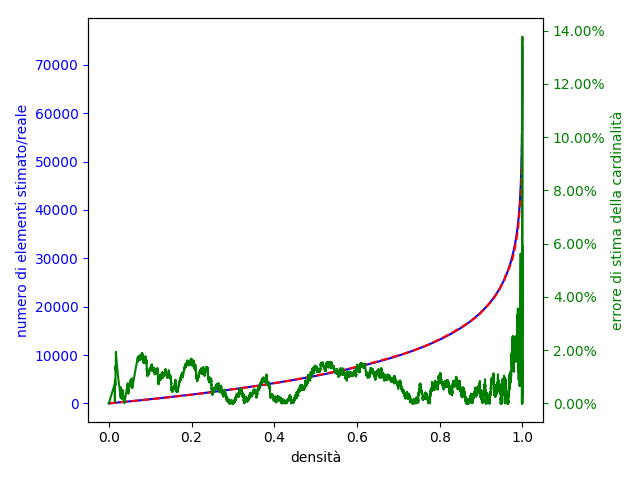
\includegraphics[width=\textwidth]{img/bloom_card_error_1h}%
		}
	\end{minipage}
	\begin{minipage}[c]{0.7\textwidth}
		\subfloat[][M=8192, K=2]{%
			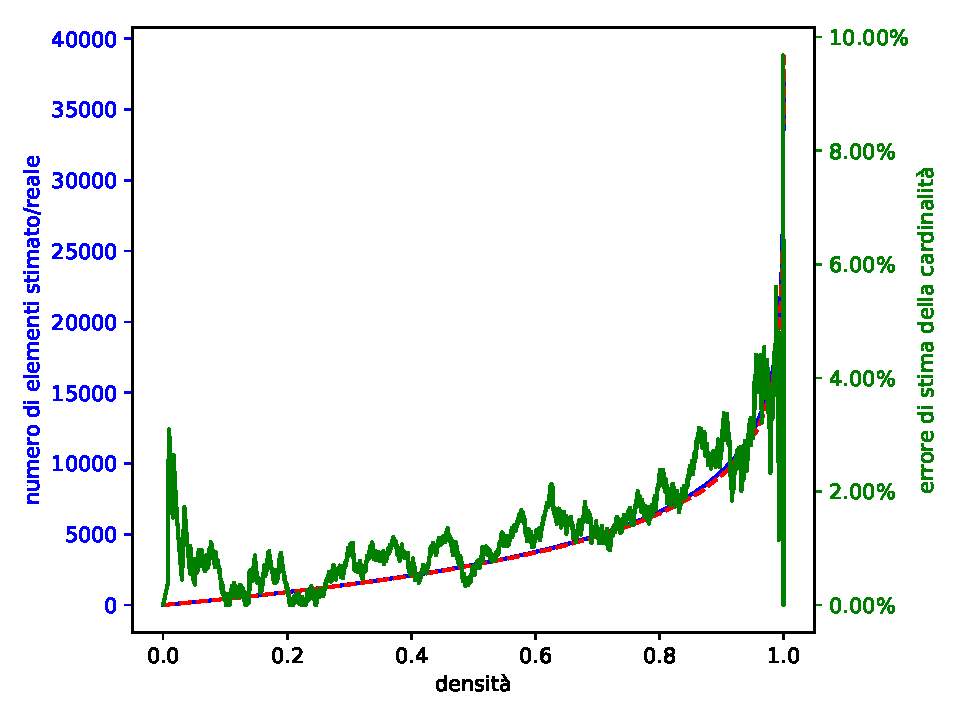
\includegraphics[width=\textwidth]{img/bloom_card_error_2h}%
		}
	\end{minipage}
	\begin{minipage}[c]{0.7\textwidth}
		\subfloat[][M=8192, K=3]{%
			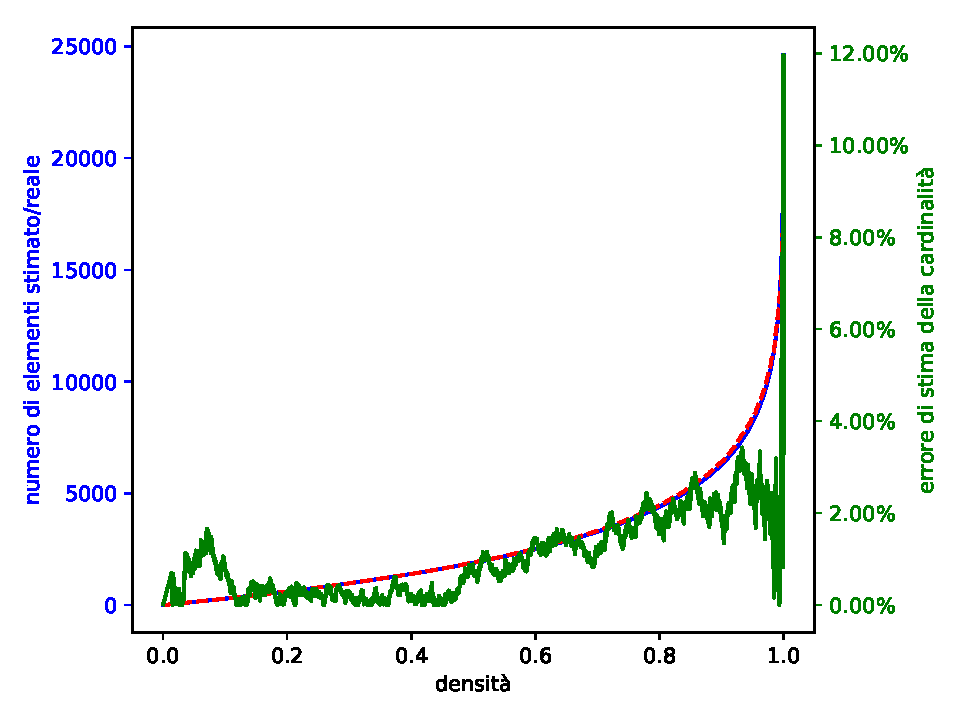
\includegraphics[width=\textwidth]{img/bloom_card_error_3h}%
		}
	\end{minipage}

	\caption{Errore commesso dall'\autoref{eq:bloomcard} per la stima della car\-di\-na\-li\-tà nei
	filtri di Bloom}
	\label{fig:bloomerror}
\end{figure}

\subsection{Unione ed intersezione}

Dati due filtri creati con gli stessi parametri ed utilizzanti le stesse funzioni di hash, è
possibile calcolare l'unione come mostrato nell'\autoref{alg:bloomunion}, semplicemente applicando
l'operazione di \cverb|OR| bit a bit agli array. Questa operazione non causa alcuna perdita di
informazione né peggioramento della probabilità di falsi positivi, poiché l'array risultante è il
medesimo che si sarebbe ottenuto aggiungendo in un solo filtro tutti gli elementi presenti nel primo
e nel secondo filtro in input.

\begin{algorithm}
\caption{Unione di due filtri di bloom}
\label{alg:bloomunion}
\begin{algorithmic}[1]
\Require $bf_1$ e $bf_2$ devono essere costruiti con gli stessi pa\-ra\-me\-tri
\Procedure{BloomUnion}{$bf_1$, $bf_2$}
	\For {$i=1$ \textbf{to} $M$}
		\State $out(i) \gets bf_1(i) \lor bf_2(i)$
	\EndFor
	\State \Return $out$
\EndProcedure
\end{algorithmic}
\end{algorithm}


È possibile in modo simile calcolare l'intersezione tra due filtri applicando l'operazione di
\cverb|AND| bit a bit agli array, come descritto nell'\autoref{alg:bloomintersection}. In questo caso
però il risultato non è ottimale: l'array risultante potrebbe contenere alcuni bit impostati a 1 che
non risulterebbero tali se si fosse creato direttamente un filtro aggiungendo solo gli elementi
facenti parte dell'intersezione e di conseguenza la probabilità di falsi positivi risultante dal
filtro intersezione è potenzialmente non ottimale.

\begin{algorithm}
\caption{Intersezione di due filtri di bloom}
\label{alg:bloomintersection}
\begin{algorithmic}[1]
\Require $bf_1$ e $bf_2$ devono essere costruiti con gli stessi pa\-ra\-me\-tri
\Procedure{BloomIntersect}{$bf_1$, $bf_2$}
	\For {$i=1$ \textbf{to} $M$}
		\State $out(i) \gets bf_1(i) \land bf_2(i)$
	\EndFor
	\State \Return $out$
\EndProcedure
\end{algorithmic}
\end{algorithm}

Supponiamo per esempio di avere due filtri che contengono rispettivamente gli elementi $\{ A, B \}$
e $\{ A, C \}$. Le funzioni di hash sugli elementi sono le seguenti:

\begin{center}
	\begin{tabular}{ l c c c }
		 & A & B & C \\
		\hline
		$h_1(x)$ & 5 & 2 & 7 \\
		$h_2(x)$ & 9 & 6 & 2 \\	
		\hline
	\end{tabular}
\end{center}

I filtri risultanti saranno i seguenti:

\begin{center}
  \begin{tabular}{*{11}{|c}|}
  	\multicolumn{1}{c}{0} & \multicolumn{1}{c}{1} & \multicolumn{1}{c}{2} &
  	\multicolumn{1}{c}{3} & \multicolumn{1}{c}{4} & \multicolumn{1}{c}{5} &
  	\multicolumn{1}{c}{6} & \multicolumn{1}{c}{7} & \multicolumn{1}{c}{8} &
  	\multicolumn{1}{c}{9} & \multicolumn{1}{c}{10} \\
    \hline
    0 & 0 & B & 0 & 0 & A & B & 0 & 0 & A & 0 \\
    \hline
  \end{tabular}
\end{center}

\begin{center}
  \begin{tabular}{*{11}{|c}|}
  	\multicolumn{1}{c}{0} & \multicolumn{1}{c}{1} & \multicolumn{1}{c}{2} &
  	\multicolumn{1}{c}{3} & \multicolumn{1}{c}{4} & \multicolumn{1}{c}{5} &
  	\multicolumn{1}{c}{6} & \multicolumn{1}{c}{7} & \multicolumn{1}{c}{8} &
  	\multicolumn{1}{c}{9} & \multicolumn{1}{c}{10} \\
    \hline
    0 & 0 & C & 0 & 0 & A & 0 & C & 0 & A & 0 \\
    \hline
  \end{tabular}
\end{center}

dove ogni cella impostata a 1 viene identificata con una lettera che si riferisce all'elemento che
l'ha impostata durante l'inserimento. 

L'insieme unione è $\{ A, B \} \cup \{ A , C \} = \{ A, B, C \}$ e il filtro risultante
dall'operazione di \cverb|OR| bit a bit, come si può vedere, è ottimale poiché è lo stesso che
avremmo ottenuto per inserimento diretto:

\begin{center}
  \begin{tabular}{*{11}{|c}|}
  	\multicolumn{1}{c}{0} & \multicolumn{1}{c}{1} & \multicolumn{1}{c}{2} &
  	\multicolumn{1}{c}{3} & \multicolumn{1}{c}{4} & \multicolumn{1}{c}{5} &
  	\multicolumn{1}{c}{6} & \multicolumn{1}{c}{7} & \multicolumn{1}{c}{8} &
  	\multicolumn{1}{c}{9} & \multicolumn{1}{c}{10} \\
    \hline
    0 & 0 & B,C & 0 & 0 & A & B & C & 0 & A & 0 \\
    \hline
  \end{tabular}
\end{center}

L'insieme intersezione è $\{ A, B \} \cap \{ A , C \} = \{ A \}$, ma il filtro risultante
dall'operazione di \cverb|AND| bit a bit è il seguente:

\begin{center}
  \begin{tabular}{*{11}{|c}|}
  	\multicolumn{1}{c}{0} & \multicolumn{1}{c}{1} & \multicolumn{1}{c}{2} &
  	\multicolumn{1}{c}{3} & \multicolumn{1}{c}{4} & \multicolumn{1}{c}{5} &
  	\multicolumn{1}{c}{6} & \multicolumn{1}{c}{7} & \multicolumn{1}{c}{8} &
  	\multicolumn{1}{c}{9} & \multicolumn{1}{c}{10} \\
    \hline
    0 & 0 & B,C & 0 & 0 & A & 0 & 0 & 0 & A & 0 \\
    \hline
  \end{tabular}
\end{center}
	
Il bit 2 rimane acceso a causa di un conflitto tra le funzioni di hash ($h_1(B) = h_2(C)$), ma
né l'elemento $B$ né l'elemento $C$ sono presenti nell'insieme intersezione. Se il filtro fosse
stato creato da zero, inserendo solamente $A$, il bit 2 risulterebbe impostato a zero.

\section{Ottimizzazione dei parametri}
\label{sec:bloomparms}

Nelle sezioni precedenti, sono stati introdotti diversi parametri che possono essere usati
per definire un filtro di Bloom:

\begin{description}[labelindent=2\parindent,labelwidth=3em]
	\item[$M$] Dimensione in bit dell'array.
	\item[$K$] Numero delle funzioni di hash (e delle sezioni).
	\item[$m$] Dimensione in bit di una sezione.
	\item[$N$] Numero di elementi presenti nel filtro.
	\item[$p$] Densità (numero di bit impostati a 1 sul totale).
	\item[$P$] Probabilità di un falso positivo.
\end{description}

Vediamo ora come è possibile ottimizzare i parametri, cercando di minimizzare $P$, la probabilità
di un falso positivo, come descritto in \cite{bloom-scalable}.

La probabilità di trovare un bit impostato a 1 in una sezione è $p$, di conseguenza la probabilità 
di un falso positivo, cioè di trovare i bit di tutte le sezioni già impostati, è:

$$ P = p^K $$

Ricordando che $M=km$, otteniamo:

$$ m = M\frac{\ln(p)}{\ln(P)} $$

e sostituendo nella formula della cardinalità, otteniamo:

$$ N \approx -M\frac{\ln(p)\ln(1-p)}{\ln(P)} $$

Supponiamo ora di fissare $M$ (dimensione del filtro) e $P$ (probabilità di un falso positivo), e di
voler cercare qual è la densità $p$ che massimizza il numero di elementi presenti nell'array. È
facile convincersi che il massimo della funzione $\ln(p)\ln(1-p)$ si trova con $p=0.5$, risultato
che ci indica che il punto di utilizzo ottimo di un filtro di Bloom è quando la densità è
esattamente al 50\%, cioè metà dei bit è impostato a 1.

Sostituendo quindi $p=0.5$ come valore ottimo, otteniamo:

$$ N \approx -M\frac{\ln(0.5)^2}{\ln(P)} $$
\begin{equation} \label{eq:bloomn}
N \approx \ceil*{M\frac{0.480453014}{|\ln(P)|}}
\end{equation}

che ci permette di calcolare il numero di elementi memorizzabili in un filtro prima di raggiungere
la densità di 0.5 e dunque la probabilità $P$ di falsi positivi richiesta. Oppure, ricavando
le altre variabili:

\begin{equation} \label{eq:bloomm}
M = \ceil*{n\frac{|\ln(P)|}{0.480453014}} 
\end{equation}
\begin{equation} \label{eq:bloomp}
P = e^{-\ln(0.5)^2\frac{M}{N}} = 0.5^{\ln(2)\frac{M}{N}} \approx 0.6185^{\frac{M}{N}}
\end{equation}

possiamo calcolare la dimensione ottimale di un filtro dato il numero di elementi che si vuole
memorizzare e la probabilità di falsi positivi attesa, oppure ancora i falsi positivi attesi
data la dimensione di un filtro e il numero di elementi inseriti. 

Inoltre, da $P = p^k$, sostituendo nuovamente $p=0.5$, possiamo ricavare:

\begin{equation} \label{eq:bloomk}
 K = \ceil*{\log_2{\frac{1}{P}}} = \ceil*{-\log_2{P}}
\end{equation}

con cui calcolare il numero ottimale di funzioni di hash per un data probabilità attesa di falso
positivo.

Vediamo ora due esempi di derivazione di parametri ottimali. 

\begin{itemize}
	\medskip

	\item Supponiamo di voler memorizzare $N=\num{25000}$ elementi in un filtro con una probabilità di
	falso positivo $P=\SI{0.5}{\percent}$; possiamo ricavare i parametri necessari in questo modo:

	$$ M = \ceil*{n\frac{|\ln(P)|}{0.480453014}} = \ceil*{25000\frac{|\ln(0.005)|}{0.480453014}} = \num{275694} $$
	$$ K = \ceil*{-\log_2{P}} = \ceil*{-\log_2{0.005}} = 8 $$

	Quindi è necessario utilizzare un filtro di $\SI{275694}{\bit} \approx \SI{33}{\kibi\byte}$ con 
	\num{8} funzioni di hash.

	\item Supponiamo di avere \SI{1}{\mebi\byte} di RAM a disposizione per creare un filtro di Bloom
	che deve memorizzare 2 milioni di elementi. Qual è il valore minimo di falso positivo che
	possiamo ottenere, e con quante funzioni di hash lo otterremo? È presto detto:

	$$ M = \num{1024 x 1024 x 8} = \num{8388608} $$
	$$ N = \num{2000000} $$
	$$ P = 0.6185 ^ \frac{M}{N} \approx 0.1463 \approx \SI{15}{\percent} $$
	$$ K = \ceil*{-\log_2{P}} = 3 $$

	Quindi possiamo arrivare ad avere circa il \SI{15}{\percent} di falsi positivi utilizzando
	\num{3} funzioni di hash.
\end{itemize}

\begin{figure}
	\centering
	\begin{minipage}[c]{\textwidth}
		\subfloat[][Numero di elementi in base alla probabilità attesa]{%
			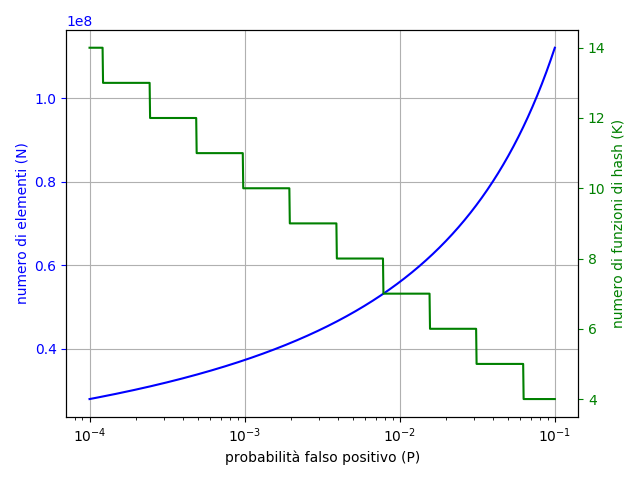
\includegraphics[width=\textwidth]{img/bloom_parms_1}%
		}
	\end{minipage}
	\qquad
	\begin{minipage}[c]{\textwidth}
		\subfloat[][Probabilità attesa in base al numero di elementi]{%
			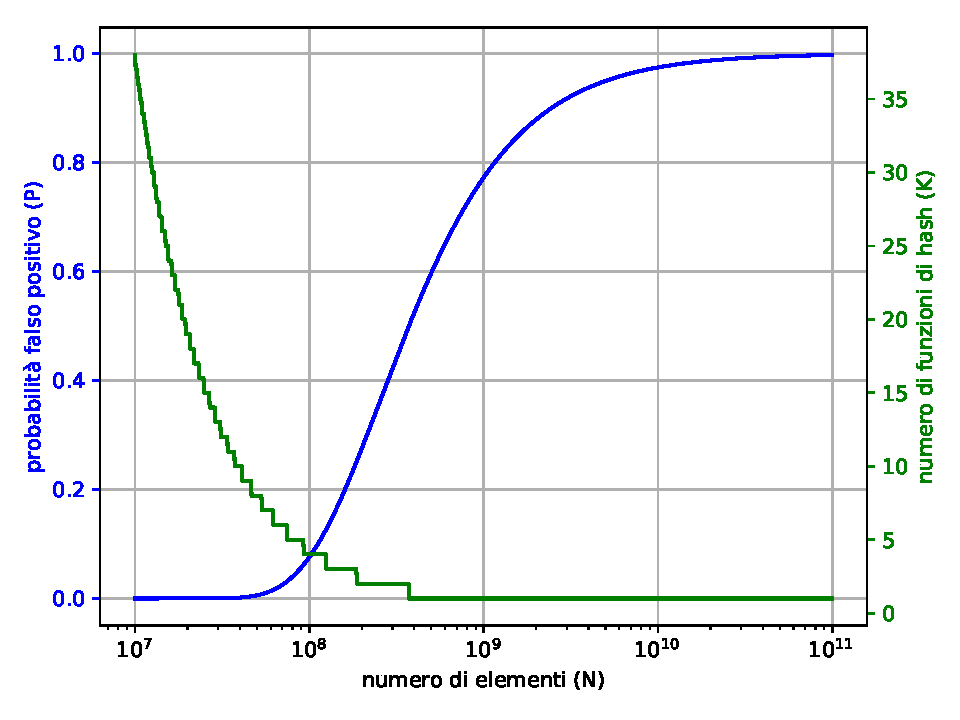
\includegraphics[width=\textwidth]{img/bloom_parms_2}%
		}
	\end{minipage}

	\caption{Andamento ottimale dei parametri in un filtro di \SI{64}{\mebi\byte}}
\end{figure}

\section{Filtri scalabili}
\label{sec:bloomscalable}

Uno dei problemi principali dei filtri così come originariamente progettati è che la struttura
dati è definita staticamente e dunque non è possibile espanderla dinamicamente in base al
numero di elementi che via via si rende necessario memorizzare. Questo limite rende complesso
l'utilizzo in diversi scenari applicativi, poiché, volendo mantenere la probabilità di un falso
positivo contenuta entro una soglia, è necessario spesso sovradimensionare il filtro a causa della 
impossibilità di prevedere il numero di elementi che sarà necessario memorizzare.

Per risolvere questo problema, \cite{bloom-scalable} propone di creare un \emph{filtro di Bloom
scalabile} (SBF) formato da uno o più filtri in catena; quando i filtri raggiungono la densità
scelta come obiettivo (di solito $p=0.5$), un nuovo filtro viene aggiunto in coda alla catena,
facendo spazio così per l'inserimento di nuovi elementi. Il test di appartenenza dovrà quindi
ricercare l'elemento all'interno di tutti i filtri della catena. 

Ogni filtro che viene creato avrà una nuova probabilità $P_j$ per i falsi positivi, seguendo una
progressione geometrica ($P_i = rP_{i-1} = r^iP_0$), in modo che la probabilità composta $P$
dell'intera catena converga verso il valore richiesto. Il fattore $r \in \interval[open]{0}{1}$ è
detto ``fattore di intensificazione'' (\emph{tighten ratio}).

La probabilità composta $P$, ottenuta ricercando l'elemento negli $l$ filtri della catena, può
essere quindi calcolata così:

$$ P = 1 - \prod_{i=0}^{l-1}(1-r^iP_0) $$

e volendo calcolare un limite superiore, possiamo ottenere:

$$ P \leq \sum_{i=0}^{l-1} r^iP_0 \leq \lim_{l \rightarrow \infty} \sum_{i=0}^{l-1} r^iP_0 =
\frac{1}{1-r}P_0 $$

Ricavando $P_0$, possiamo calcolare il valore di probabilità di falsi positivi che deve avere
il primo filtro della catena, in base al fattore di intensificazione $r$ e la probabilità finale
attesa $P$:

\begin{equation} \label{eq:p0fromp}
P_0 = (1-r)P
\end{equation}

Possiamo anche calcolare il numero ottimale di funzioni di hash che deve usare ogni filtro nella
catena:

$$ k_0 = -\log_2{P_0} $$
$$ k_i = -\log_2{P_i} = -\log_2{(r^iP_0)} = k_0 - i \log_2{r} $$

Per quanto concerne invece la dimensione $M_i$ dei filtri, è consigliabile utilizzare anche qui
una progressione geometrica (il cui fattore è chiamato $s$), che si adatta velocemente ad una
crescita importante di elementi nel filtro senza aumentare troppo la lunghezza della catena (che
impatterebbe sulla velocità del test di appartenenza). 

Per quanto concerne i valori ottimali dei parametri $r$ e $s$, rimandiamo a \cite{bloom-scalable} per
l'analisi sperimentale che mostra che i valori ottimali di $r$ sono $r \in \interval{0.8}{0.9}$,
mentre il parametro $s$ può essere usato normalmente con valore \num{2}, aumentando magari a \num{4}
se si prevede un numero molto elevato di elementi.


\appendix
\appendixpage
\chapter{Codice sorgente}

\section{Esempio di stored procedure in Redis}

Il seguente listato mostra una stored procedure scritta in LUA che dato un insieme ordinato
\cverb|paying-users| in cui le stringhe sono gli ID degli utenti di un sistema, e il punteggio
associato è il totale speso dall'utente nell'applicazione, calcola qual è la media di spesa degli
utenti ``premium'', cioè che hanno speso più di \SI{1000}{\EUR}.

Si veda la \autoref{sec:redis:lua} per maggiori informazioni.

\sourcecode[language={[5.0]Lua}]{code/zsetaverage.lua}


\section{Calcolo dell'errore di cardinalità di un filtro di Bloom}

Il seguente listato effettua una simulazione di calcolo dell'errore di cardinalità in un filtro
di Bloom di \SI{8192}{\bit}, con $2$ funzioni di hash.

Si veda la \autoref{sec:bloomcard} per maggiori informazioni.

\sourcecode[language=Python]{code/cardinality.py}


\section{Calcolo dei parametri ottimali di un filtro di Bloom}

I seguenti listati effettuano il calcolo dei parametri ottimali per un filtro di Bloom da 64 MiB.

Si veda la \autoref{sec:bloomparms} per maggiori informazioni.

\sourcecode[language=Python]{code/bloomparms1.py}
\sourcecode[language=Python]{code/bloomparms2.py}


\section{Modifica al database Redis}
\label{sec:modredis}

I seguenti listati mostrano la parte principale della modifica al database Redis:
l'implementazione del filtro di Bloom, e i test automatizzati che verificano la correttezza
del codice. Si veda la \autoref{sec:patchexplain} per una descrizione dettagliata di questo codice.

\subsection{Implementazione dei filtri di Bloom}
\sourcecode[language=C]{code/bloom.h}
\sourcecode[language=C]{code/bloom.c}

\subsection{Test di unità}
\sourcecode[language=tcl]{code/bloom.tcl}

\subsection{Analisi dei parametri del filtro scalabile}
\sourcecode[language=Python]{code/scalingbloomparms.py}

\begin{thebibliography}{99}

\bibitem{corbellini}
	A. Corbellini, C. Mateos, A. Zunino, D. Godoy, S. Schiaffino - 
	\emph{Persisting Big Data: The NoSQL landscape} - 
	ISISTAN (CONICET-UNCPBA) Research Institute1, UNICEN University, Campus Universitario, Tandil B7001BBO, Argentina - 
	2016

\bibitem{nascita}
	Stefano Bernardi - 
	\emph{An interview with Salvatore Sanfilippo, creator of Redis, working out of Sicily} - 
	\url{http://www.eu-startups.com/2011/01/an-interview-with-salvatore-sanfilippo-creator-of-redis-working-out-of-sicily/}

\bibitem{murmur2flaw}
	\emph{MurMur2 Hash Function Flaw} -
	\url{https://github.com/aappleby/smhasher/wiki/MurmurHash2Flaw}

\bibitem{select}
	\emph{Waiting for Input or Output} - 
	The GNU C Library - 
	\url{https://www.gnu.org/software/libc/manual/html_node/Waiting-for-I_002fO.html}

\bibitem{epoll}
	\emph{epoll(4)} - 
	Linux Man page - 
	\url{https://linux.die.net/man/4/epoll}

\bibitem{aws-latency}
	Steve Newman -
	\emph{Three latency anomalies} - 
	Am I stronger Yet? - 
	\url{http://amistrongeryet.blogspot.it/2010/04/three-latency-anomalies.html}

\bibitem{lua-angry}
	Ansca Inc. -
	\emph{Lua: the lingua franca of iPhone games} -
	Company blog -
	\url{https://web.archive.org/web/20120502071633/http://blog.anscamobile.com/2010/04/lua-the-lingua-franca-of-iphone-games/} -
	Archived by the Internet Web Archive

\bibitem{lua-wow}
	\emph{Lua} -
	WOWWiki on Wikia -
	\url{http://wowwiki.wikia.com/wiki/Lua}

\bibitem{tcp-cork}
	Chris Baus -
	\emph{TCP\_CORK: More than you ever wanted to know} -
	\url{http://baus.net/on-tcp_cork}

\bibitem{tcp-cork-redispy}
	Sorgenti di redispy - connection.py -
	\url{https://github.com/andymccurdy/redis-py/blob/8a186ebd9cecf466624803bdf215030158c7c776/redis/connection.py\#L517}

\bibitem{hyperloglog}
	Philippe Flajolet, Éric Fusy, Olivier Gandouet, e Frédéric Meunier -
	\emph{HyperLogLog: the analysis of a near-optimal cardinality estimation algorithm} -
	2007 Conference on Analysis of Algorithms, AofA 07 -
	\url{http://algo.inria.fr/flajolet/Publications/FlFuGaMe07.pdf}

\bibitem{hyperloglog-plusplus}
	Stefan Heule, Marc Nunkesser e Alexander Hall -
	\emph{HyperLogLog in Practice: Algorithmic Engineering of a State of The Art Cardinality Estimation Algorithm} -
	EDBT/ICDT ’13 March 18 - 
	\url{https://static.googleusercontent.com/media/research.google.com/en//pubs/archive/40671.pdf}

\bibitem{hyperloglog-explain}
	Juan Lopes -
	Answer to question: \emph{How does the HyperLogLog algorithm work?} -
	Stack Overflow -
	\url{https://stackoverflow.com/a/12734343/118015}

\bibitem{fb-mau}
	Josh Cosentine -
	\emph{Facebook now has 2 billion monthly users... and responsibility} -
	TechCrunch -
	\url{https://techcrunch.com/2017/06/27/facebook-2-billion-users/}

\bibitem{lasvegas}
	László Babai -
 	Monte-Carlo algorithms in graph isomorphism testing -
 	Eötvös University, Budapest, Hungary

\bibitem{bloomfilters}
	Burton H. Bloom -
	Space/Time Trade-offs in Hash Coding with Allowable Errors -
	Commun. ACM 13(7): 422-426 -
	1970

\bibitem{golomb}
	Golomb-Rice Coding -
	\url{https://en.wikipedia.org/wiki/Golomb_coding}

\bibitem{golomb-safebrowsing}
	Google Safe Browsing - Compression
	\url{https://developers.google.com/safe-browsing/v4/compression}

\bibitem{bloomnetwork}
	Andrei Broder and Michael Mitzenmacher -
	\emph{Network Applications of Bloom Filters: A Survey} -
	Internet Mathematics Vol. 1, No. 4: 485-509
	\url{http://www.eecs.harvard.edu/~michaelm/postscripts/im2005b.pdf}

\bibitem{bloomproxy}
	L. Fan, P. Cao, J. Almeida, and A. Z. Broder. -
	\emph{Summary Cache: A Scalable Wide-Area Web Cache Sharing Protocol.} -
	IEEE/ACM Transactions on Networking 8:3 (2000), 281—293.

\bibitem{bloomakamai}
	Maggs, Bruce M.; Sitaraman, Ramesh K. -
	\emph{Algorithmic nuggets in content delivery} -
	SIGCOMM Computer Communication Review, New York, NY, USA -
	ACM, 45 (3): 52–66, doi:10.1145/2805789.2805800 -
	July 2015

\bibitem{bloomdoublehash}
	Dillinger, Peter C.; Manolios, Panagiotis - 
	\emph{Bloom Filters in Probabilistic Verification} -
	Proceedings of the 5th International Conference on Formal Methods in Computer-Aided Design, Springer-Verlag, Lecture Notes in Computer Science 3312

\bibitem{bloomscalable}
	Paulo Sergio Almeida, Carlos Baquero, Nuno Preguiça, David Hutchison -
	\emph{Scalable Bloom Filters} -
	Information Processing Letters archive Volume 101 Issue 6, pages 255-261 -
	March 2007 -
	\url{http://gsd.di.uminho.pt/members/cbm/ps/dbloom.pdf}

\bibitem{lemirereduction}
	Daniel Lemire -
	\emph{A fast alternative to the modulo reduction} -
	Daniel Lemire's blog -
	June 2016 -
	\url{https://lemire.me/blog/2016/06/27/a-fast-alternative-to-the-modulo-reduction/}

\end{thebibliography}

%--------------------------------------------------------------
\end{document}
%--------------------------------------------------------------
